
\documentclass[10pt]{article} % For LaTeX2e
%\usepackage{tmlr}
% If accepted, instead use the following line for the camera-ready submission:
\usepackage[accepted]{tmlr}
% To de-anonymize and remove mentions to TMLR (for example for posting to preprint servers), instead use the following:
%\usepackage[preprint]{tmlr}

% Optional math commands from https://github.com/goodfeli/dlbook_notation.
\input{math_commands.tex}

\usepackage{hyperref}
\usepackage{url}

% Recommended, but optional, packages for figures and better typesetting:
\usepackage{microtype}
\usepackage{graphicx}
\usepackage{subcaption}
\usepackage{booktabs} % for professional tables
\usepackage{multirow}
\usepackage{rotating} % for the sideways combined-results table (draws content
                       % genuinely rotated, unlike pdflscape's /Rotate flag which
                       % many viewers/printers don't honor)
\usepackage{xcolor}
\usepackage{tcolorbox}
\tcbuselibrary{breakable} % Required for page-splitting
\usepackage{mathrsfs}
\usepackage{enumitem}
\usepackage{hyperref}
\usepackage{amsmath}
\usepackage{amssymb}
\usepackage{bbm}
\usepackage{mathtools}
\usepackage{amsthm}
\usepackage{float}
\usepackage[capitalize,noabbrev]{cleveref}

\crefname{equation}{}{}
\Crefname{equation}{}{}

%%%%%%%%%%%%%%%%%%%%%%%%%%%%%%%%
% THEOREMS
%%%%%%%%%%%%%%%%%%%%%%%%%%%%%%%%
\theoremstyle{plain}
\newtheorem{theorem}{Theorem}[section]
\newtheorem{proposition}[theorem]{Proposition}
\newtheorem{lemma}[theorem]{Lemma}
\newtheorem{corollary}[theorem]{Corollary}
\theoremstyle{definition}
\newtheorem{definition}[theorem]{Definition}
\newtheorem{assumption}[theorem]{Assumption}
\theoremstyle{remark}
\newtheorem{remark}[theorem]{Remark}

\title{Certifying global optima in non-convex optimization problems using deep neural networks}


% Authors must not appear in the submitted version. They should be hidden
% as long as the tmlr package is used without the [accepted] or [preprint] options.
% Non-anonymous submissions will be rejected without review.

\author{\name Charles Gulian \email charlesgulian@berkeley.edu \\
      \addr Industrial Engineering \& Operations Research Dept.\\
      University of California, Berkeley
      \AND
      \name Ying Chen \email ying-chen@berkeley.edu \\
      \addr Industrial Engineering \& Operations Research Dept.\\
      University of California, Berkeley
      \AND
      \name Javad Lavaei \email lavaei@berkeley.edu\\
      \addr Industrial Engineering \& Operations Research Dept.\\
      University of California, Berkeley}

% The \author macro works with any number of authors. Use \AND 
% to separate the names and addresses of multiple authors.

\newcommand{\fix}{\marginpar{FIX}}
\newcommand{\new}{\marginpar{NEW}}

\def\month{MM}  % Insert correct month for camera-ready version
\def\year{YYYY} % Insert correct year for camera-ready version
\def\openreview{\url{https://openreview.net/forum?id=XXXX}} % Insert correct link to OpenReview for camera-ready version


\begin{document}

\maketitle

\begin{abstract}
Solving non-convex optimization problems in real-time is a ubiquitous challenge in cyber-physical systems engineering. 
Most fast solvers rely on heuristics or local search methods that are not guaranteed to converge to global optima for non-convex problems.
On the other hand, slow, exact solvers such as convexification techniques or branch-and-bound are typically too slow to use in online settings. 
We propose a framework that bridges between fast and slow solvers via \textit{neural network-based optimality certificates}. 
The framework leverages slow, exact solvers \textit{offline} to learn the optimal value of parametric non-convex problems using deep neural networks. 
The neural network's predictions are then used \textit{online} to certify global optimality of feasible solutions obtained from fast, local or heuristic solvers. 
We demonstrate the power of the proposed framework on several realistic problems from power systems, robotics, signal processing, and integer optimization. We also demonstrate its application to speed up traditional non-convex solvers such as branch-and-bound. Our results indicate that neural networks can effectively identify suboptimal solutions in real-time, potentially leading to improved solution accuracy without compromising speed.
\end{abstract}

\section{Introduction}

%Solving non-convex optimization problems efficiently is a ubiquitous challenge in many engineering disciplines.
Quickly solving non-convex optimization problems is a ubiquitous challenge in many engineering disciplines. 
In power system operations, the AC optimal power flow (AC-OPF) problem is solved approximately every five minutes to balance time-varying load and generation \citep{van2021machine}.
Robots and autonomous vehicles solve non-convex route planning problems to reach targets and avoid collisions in changing environments \citep{ahmadi2016some}. 
In digital communication networks, signals are transmitted and recovered over noisy channels at millisecond timescales \citep{samuel2017deep}. 
The list of applications goes on.

Many non-convex optimization solvers rely on fast but approximate algorithms or heuristics that may return suboptimal solutions, which incur higher cost, waste resources, or reduce safety margins unnecessarily. Therefore, being able to quickly certify the optimality of solutions obtained by fast solvers could potentially be extremely valuable. For example, operating the California power system costs roughly \$10-15 billion/year and emits roughly 40 MMT/year of greenhouse gases \citep{CAISO_DMM_2023}. Even a 0.1\% average improvement in operating efficiency could yield cost savings of \$10-15 million/year or reduce emissions by 40,000 MT/year.

However, certifying global optima is difficult for non-convex problems. Unlike in convex optimization, global optima in non-convex problems may not be certified from local information such as the KKT conditions \citep{boyd2004convex}. In fact, certifying global optima in non-convex problems is NP-hard in general \citep{murty1985some}. 
A major challenge is the possible presence of multiple local optima where local search and gradient-based methods can get stuck. Stochastic search, ensemble methods, and various heuristic algorithms seek to overcome this issue by exploring the solution space more broadly and injecting noise to escape poor local optima \citep{dauphin2014identifying, kumar2020test}. Recently, machine learning-based solvers have also been used to obtain good solutions to non-convex problems \citep{donti2021dc3, jiang2024advancements}. Despite their impressive speed and accuracy, these methods are not guaranteed to converge to global optima, leading to worse outcomes in terms of cost, efficiency, or safety in real-world application settings.

Slow, exact solvers with global optimality guarantees for non-convex problems have also been studied extensively. These methods include spatial branch-and-bound solvers such as BARON and Couenne \citep{tawarmalani2005polyhedral, belotti2009branching}, as well as convexification methods such as sum-of-squares hierarchies and the reformulation-linearization technique \citep{lasserre2001global, ahmadi2019dsos, rudi2020finding, sherali2013reformulation}. Spatial branch-and-bound iteratively partitions the search space and solves convex relaxations over each subregion to obtain progressively tighter lower bounds. Convexification replaces non-convex objectives or constraints with convex outer-approximations, often in lifted or higher-dimensional spaces. Convex relaxations are solvable in polynomial time and provide global lower bounds for the optimal value of the original non-convex problem \citep{boyd2004convex}.
%(as do the subproblems of spatial branch-and-bound over each subregion).
%When the optimal objective function values are equal, the convex relaxation is said to be \textit{exact} and the method is called \textit{convexification}.
However, solving a convex relaxation can be exponentially slower than solving the original problem with local search or machine learning-based solvers, as convexification may introduce many more variables and constraints. Therefore, despite their power, these approaches scale poorly with problem size and are impractical to use in real-time applications.

We propose a framework which leverages machine learning to assist in non-convex optimization by certifying global optima in real-time. Specifically, we train deep neural networks to approximate the optimal value function of parametric non-convex problems. 
Convexification methods provide tight lower bounds on the optimal value of many problem instances, which are solved in parallel offline to obtain training data. The neural network predictions are then compared with the objective value of feasible solutions obtained from fast, local solvers to approximately certify global optimality.
%Convexification is used offline to obtain training data for learning the optimal value function, while the trained neural network is used online to certify optimality of feasible solutions obtained by fast solvers.
Our approach thus distills the power of convexification methods into \textit{neural network optimality certificates} that can be deployed in real-time application settings.

%\subsection{Parametric Non-Convex Optimization}

% We are concerned with parametric non-convex optimization problems of the form
% \begin{align}
%     v(p) := ~\min_{x \in \mathbb{R}^n}~&f(x; p) \label{eq:parametric_opt} \\
%     \text{s.t.}~& g_i(x; p) \leq 0, \quad i = 1, 2, ... , m \nonumber \\
%     & h_i(x;p) = 0, \quad i = 1, 2, ..., l \nonumber
% \end{align}
% in which the parameter $p$ takes values in $\Phi \subseteq \mathbb{R}^d$. In time-varying optimization, $p$ takes a sequence of values $(p_t)_{t=1}^{\infty}$ with $p_t \in \Phi$ for all $t = 1, 2, 3, ...$. We suppose that the objective function and/or at least one of the constraints is non-convex, making \eqref{eq:parametric_opt} a non-convex problem.

% Time-varying non-convex optimization is ubiquitous in cyber-physical systems engineering, machine learning, finance, signal processing, and other domains. For instance, power system operators optimize generator setpoints every 5-15 minutes by solving non-convex AC optimal power flow (AC-OPF) parameterized by time-varying load or net load. Financial engineers solve non-convex portfolio optimization problems parameterized by time-varying market signals and asset prices. Signal processing engineers rapidly solve multi-input multi-output (MIMO) detection problems with time-varying communication signals. The list goes on.

% Local search methods such as gradient descent and interior point methods are often used to solve non-convex problems in real-time, even though they are not guaranteed to obtain global minima (reference). Unlike convex problems, non-convex problems may have multiple local minima and disconnected feasible regions where local search methods can get ``stuck." Indeed, non-convex optimization is NP-hard in general, though many approaches have been developed to address its inherent challenges (reference). These include heuristics such as simulated annealing and evolutionary algorithms, which are designed to escape poor local minima by exploring the solution space more globally ~\citep{dauphin2014identifying, kumar2020test}. In addition, specialized first-order methods, such as stochastic gradient descent with momentum and adaptive learning rates have been applied with some success in machine learning tasks ~\citep{moreira1995neural, yuan2022new}. However, these methods typically lack global optimality guarantees as well.

% %\subsection{Convex Relaxation Methods}

% A powerful approach for globally solving non-convex problems is convex relaxation ~\citep{Tropp2006, Chandrasekaran_2012}. The basic idea is to replace the non-convex objective or feasible set of \eqref{eq:parametric_opt} with a convex outer-approximation, perhaps in a lifted space. For example, let $\text{epi}(f;p) := \{(x,t) \in \mathbb{R}^{n+1} : x ~\text{feasible for \eqref{eq:parametric_opt}}, ~ f(x;p) \leq t\}$. A convex relaxation of \eqref{eq:parametric_opt} is:
% \begin{align}
%     \tilde{v}(p) = \min_{(x,t)\in \mathbb{R}^{n+1}} \{t : (x,t) \in \text{conv}(\text{epi}(f;p))\} \label{eq:convex_epigraph_reformulation}
% \end{align}
% We denote the value function of a convex relaxation as $\tilde{v}(p)$. A convex relaxation is called exact for a particular $p$ if $\tilde{v}(p) = v(p)$. The convex hull epigraph reformulation \eqref{eq:convex_epigraph_reformulation} is exact for all $p \in \Phi$, but is not easy to construct in general. Indeed, constructing the convex hull of $\text{epi}(f;p)$ may be just as hard as solving the original non-convex problem (reference). Practical convexification techniques seek convex outer-approximations of the objective function and feasible set with simple representations, albeit possibly in higher dimensional or more complicated spaces.

% Convex relaxation has been used in a variety of domains to solve non-convex problems. In combinatorial optimization, Goemans and Williamson (1994) famously use semidefinite relaxation and randomization techniques to develop an approximation algorithm for the max-cut problem. Bienstock (2004) constructs an approximate extended linear formulation of the 0-1 knapsack problem with a polynomial number of variables and constraints. In polynomial optimization, the Lasserre hierarchy constructs a sequence of semidefinite relaxations which become exact at high orders under a mild sufficient condition. Sojoudi and Lavaei (2014) provide sufficient conditions for the exactness of semidefinite and second-order cone relaxations of a large class of non-linear optimization problems. In power systems engineering, Lavaei and Low (2012) study a semidefinite relaxation of the AC-OPF problem and provide sufficient conditions for its exactness. See Low (2014) for a review of convex relaxations of optimal power flow. Josz and Molzahn (202?) study higher order semidefinite relaxations of AC-OPF, which are generally tighter than first-order semidefinite relaxations but much larger and slower to solve. 

% Indeed, a common theme is that the size of the convex relaxation may be orders of magnitude larger than the original problem, making these techniques all but impractical for use in online settings. For instance, to approximate the 0-1 knapsack polytope with $n$ items to within a factor of $\epsilon$, Bienstock (2004)'s extended linear formulation would require $\mathcal{O}(\epsilon^{-1}n^{1+\lceil 1/\epsilon \rceil})$ variables and $\mathcal{O}(\epsilon^{-1}n^{2+\lceil 1/\epsilon \rceil})$ constraints. As another example, for a polynomial optimization problem in $n$ variables, the decision variable of the order-$d$ Lasserre hierarchy SDP is a $\binom{n+d}{d} \times \binom{n+d}{d}$ symmetric positive semidefinite matrix. However, as we shall demonstrate, the global optimality guarantees of convex relaxations may be exploited in offline settings -- for example, to learn the value function $v(p)$ of a parametric non-convex problem.

% %\subsection{Machine Learning for Solving AC-OPF}

% An alternative approach which has garnered strong interest is the use of machine learning to assist in solving optimization problems. Examples of such applications are numerous, but we shall focus our review on machine learning applications for solving AC-OPF and related problems in power systems, as this is the motivating application of our work.

% First, we note that practical experience and some theoretical work has shown that spurious local minima are rare in realistic AC-OPF instances. Therefore AC-OPF is frequently solved to global optimality using only local search methods (reference). However, there are well-known AC-OPF instances with exponentially many disconnected feasible regions and local minima. Therefore, certifying the global optimality of AC-OPF solutions remains an important challenge.

% The goal of many machine learning-assisted solvers is to improve speed and quality of obtained solutions over traditional AC-OPF solvers.
% Some works have focused on learning to map the time-varying parameters of AC-OPF directly to optimal solutions. Zhang et al. (2021) train input convex neural networks (ICNNs) to learn the value function of parametric DC-OPF, and exploit the underlying problem structure to recover optimal solutions from the ICNN predictions. Similarly, Singh et al. (2021) and Pan et al. (2022) train neural networks to directly predict optimal solutions of parametric AC-OPF. Baker (2019) proposes to use machine learning-predicted AC-OPF solutions as warm starts for local search solvers. Chen et al. (2020) use ICNNs to assist in voltage regulation of distribution networks, while Pineda et al. (2024) use machine learning to assist in solving the DC optimal transmission switching problem.

% Though these approaches have been demonstrated to achieve good performance on  their respective target problems, but many lack global optimality guarantees (indeed, some direct solution mappings lack even feasibility guarantees). A key challenge is that optimal solution mappings are high dimensional and discontinuous, and therefore are difficult to learn (reference: Pan et al. 2022).

\subsection{Contributions}

We make the following contributions in this work.
\begin{itemize}[itemsep=2pt, parsep=1pt]
    \item We propose a novel machine learning framework that uses deep neural networks to certify global optima in non-convex optimization problems.
    \item We use convexification techniques to obtain tight lower bounds on the optimal value of non-convex problems, and thus obtain training data for our neural networks.
    \item We use split conformal calibration to obtain probabilistic guarantees for certification accuracy.
    \item We demonstrate the efficacy of our framework in several realistic experiments.
\end{itemize}

% We train neural networks to predict the optimal objective function value of non-convex optimization problems and thus certify optimality of solutions in real-time.
% A key feature of our approach is the use of convexification techniques to develop training data sets. Convexification provides a reliable way to globally solve non-convex problems. Given a parametric non-convex problem, we randomly sample pairs of problem parameters and optimal objective function values by solving an exact convex relaxation of the problem. Our approach thus shifts the computational burden of globally solving non-convex problems to an offline learning setting. 

% We are able to distill the power of convexification methods into neural networks, which can certify the optimality of solutions obtained by other solvers in real-time.

% Furthermore, we explore the intriguing possibility of enforcing structural properties of the value function in the neural network architecture and training process. For example, the value functions of certain parametric non-convex problems can be shown to be convex or positively homogeneous. We use input convex / scale invariant neural network (ICNN/SINN) architectures to improve prediction accuracy and even directly solve some non-convex problems.

% We propose to train neural networks to predict the value function $v(p)$ of time-varying non-convex optimization problems and thus certify the optimality of solutions obtained by local search methods or other solvers. Of course, the properties of the value function depend heavily on the parameterization of the problem, but in many practical examples of parametric non-convex optimization, $v(p)$ is continuous and sometimes even convex in $p$. 
% %(For example, if problem \eqref{eq:parametric_opt} admits an exact convex relaxation for all $p \in \Phi$ with value function $\tilde{v}(p) \equiv v(p)$, and if $\tilde{v}(p)$ is convex, then $v(p)$ is convex as well.)
% Therefore, the value function $v(p)$ is generally an easier learning target compared to, e.g., learning direct solution mappings. 

% Furthermore, we propose to use convexification techniques to develop training data sets for learning the value function. Convexification provides a robust way to globally solve non-convex problems. Given an exact convex relaxation of \eqref{eq:parametric_opt}, we propose to randomly sample pairs of parameters and optimal objective function values $(p, v(p)) \in \Phi \times \mathbb{R}$ to develop training data sets, where $v(p)$ is obtained by solving the convex relaxation.
% Our proposed approach shifts the computational burden of obtaining high quality (near-globally optimal) solutions to an offline learning problem. The power of convex relaxation techniques may thus be distilled into machine learning models, which can assist in online optimization settings.

% Our main contribution is conceptual in nature: we do not provide a single, specific framework for incorporating neural network-based optimality certificates into solution algorithms because many such frameworks are possible. However, we demonstrate the possibility of such approaches by training neural networks to approximate the value functions of several parametric non-convex problems.

\subsection{Paper Outline}

In Section \ref{sec:related-topics}, we give an overview of related topics. In Section \ref{sec:approach}, we describe our framework and demonstrate it on a simple non-convex problem. In Section \ref{sec:experiments}, we present results from several numerical experiments. In Section \ref{sec:discussion}, we weigh the strengths and weaknesses of our framework. We conclude our work in Section \ref{sec:conclusion}.

\subsection{Notation and Preliminaries}

Throughout this paper, we denote scalars with unbolded lower-case letters $z$, vectors (and vector-valued functions) with bolded lower-case letters $\mathbf{z}$, and matrices with unbolded capital letters $Z$. We use $\| \cdot \|$ to denote the Euclidean norm and $| \cdot |$ to denote the absolute value norm. 
%We use $\mathbb{E}_\xi[\, \cdot \,]$ or $\mathbb{P}_\xi(\cdot)$ to denote expected value or event probability with respect to the distribution of a random variable $\xi$; if the context is obvious, we occasionally drop the dependence on $\xi$ from the subscript.

\section{Related Topics} \label{sec:related-topics}

\subsection*{Parametric Non-Convex Optimization}

We are concerned with parametric non-convex optimization problems of the form
\begin{equation}
\label{prob:nonconvex}
\begin{aligned}
    v(\bm{\theta}) ~=~ \min_{x \in \mathcal{X}} \quad & f(\mathbf{x}\,;\bm{\theta}) \\
    \text{s.t.} \quad & \mathbf{x} \in \mathcal{C}(\bm{\theta})
\end{aligned}
\end{equation}
where $\mathcal{C}(\bm{\theta}) = \{\mathbf{x} \in \mathbb{R}^n: \mathbf{c}(\mathbf{x} \,; \bm{\theta}) = \mathbf{0}\}$ is a feasible set parameterized by $\bm{\theta} \in \Theta$. We assume that the objective function $f(\cdot\,; \bm{\theta})$ is non-convex or that the constraint functions $\mathbf{c}(\cdot\,;\bm{\theta})$ are nonlinear, making problem \cref{prob:nonconvex}{}{} a non-convex optimization problem. The parameter $\bm{\theta}$ typically represents some time-varying context or input to the optimization problem, such as electricity demand in optimal power flow or vehicle sensor data in route planning. Parametric problems are often encountered in cyber-physical engineering settings where a fixed non-convex problem must be solved repeatedly at high frequency for time-varying input data or parameters.

Non-convex problems are an extremely broad class of optimization problem. They are frequently encountered in real-world settings, and yet are notoriously difficult to solve. In fact, because general non-convex problems are NP-hard to solve, most successful solvers rely on bespoke algorithms tailored to specific problem classes; there are few generalist strategies. Indeed, designing efficient solvers for specific non-convex problems has remained an extremely active area of research in computer science and operations research for many years.

Despite their often impressive performance, fast non-convex solvers often lack guarantees of finding globally optimal solutions.
Our goal in this work is to train deep neural networks to quickly \textit{certify} global optima in non-convex problems.
The neural networks are trained to predict the optimal value $v(\bm{\theta})$ of a parametric non-convex problem. Their predictions may therefore be compared with the objective value of any feasible solution $\hat{\bm{x}} \in \mathcal{C}(\bm{\theta})$ to estimate its optimality gap and thus certify whether $\hat{\bm{x}}$ is near-globally optimal.
Our framework exploits convexification techniques and conformal prediction theory to provide probabilistic guarantees on the quality of a given solution and the accuracy of our certificates. 
The framework therefore \textit{complements} the extensive body of work in non-convex optimization that has developed efficient solvers for a host of specific problems.

% % Move to framework section
% Because global solvers are too slow for these budgets, practitioners overwhelmingly rely on fast local search and problem-specific heuristics that return feasible but possibly suboptimal solutions, with no guarantee of global optimality and no accompanying certificate of quality. Our aim is not to replace these solvers, but to \emph{certify} the solutions they produce. We exploit the repetitive structure of the parametric setting by shifting the burden of global optimization offline: we solve many instances exactly using slow convex relaxations, learn the optimal value function $v(\bm{\theta})$ with a neural network, and use the learned value together with a conformal calibration step to certify online whether a fast solver's solution is $\delta$-optimal. In this way our framework is complementary to existing heuristic and machine learning-based solvers---it supplies the optimality guarantee they lack, without sacrificing their speed at deployment time.

\subsection*{Machine Learning-Based Solvers}

Machine learning-based solvers for non-convex problems have been proposed in a growing number of application areas, including power systems optimization, digital communications, and integer programming \citep{van2021machine, samuel2017deep, bertsimas2022online}. Machine learning-based solvers often achieve very good performance on their respective target problems, and have been shown to be faster and more accurate than local search and heuristic algorithms in many cases. They appear to be promising alternatives to conventional solvers, yet they also suffer from the inability to guarantee or certify global optimality of obtained solutions. As a result, machine learning-based solvers have not been widely integrated into safety-critical applications \citep{sun2023online}. It remains an important challenge to develop similarly fast and accurate methods to \textit{certify} optimal solutions obtained from machine learning-based solvers.

There are several approaches to designing machine learning-based solvers. One of the most common, which includes solvers such as \textit{DeepOPF} \citep{pan2022deepopf}, seeks to directly learn a mapping from parameters to optimal solutions of a non-convex problem. Machine learning-based solvers may be trained using supervised or self-supervised learning. In the former, the model is trained to directly minimize squared error loss between the predicted and true optimal solution. For models $\hat{\mathbf{x}}(\cdot): \Theta \to \mathbb{R}^n$ in class $\mathcal{M}$, supervised learning solves
\begin{equation}
\begin{aligned}
    \min_{\hat{x}(\cdot) \in \mathcal{M}}~ \mathbb{E}_\theta\, \| \hat{\mathbf{x}}(\bm{\theta}) - \mathbf{x}^*(\bm{\theta})\|^2
\end{aligned}
\end{equation}
where the expectation is taken with respect to some probability measure over $\Theta$ and $\mathbf{x}^*(\bm{\theta})$ is an optimal solution for problem \cref{prob:nonconvex}{}{}.
In self-supervised learning, the model is trained to directly minimize the objective, usually with some form of regularization to promote feasibility of predicted solutions.
\begin{equation}
\begin{aligned}
    \min_{\hat{x}(\cdot) \in \mathcal{M}}~ \mathbb{E}_\theta \left[ \, f(\hat{\mathbf{x}}(\bm{\theta})\,; \bm{\theta}) + \rho \, \|\mathbf{c}(\hat{\mathbf{x}}(\bm{\theta})\,; \bm{\theta})\|^2 \,\right]
\end{aligned}
\end{equation}
The advantage of this approach is that it does not require labeled training data, which are expensive to obtain as it requires solving many non-convex optimization problems. A major challenge in either approach is that optimal solution mappings are high dimensional, nonlinear, and often discontinuous functions that are difficult to approximate well \citep{pan2022deepopf}. Furthermore, it is difficult to balance optimality and feasibility conditions during training \citep{park2023self}.

Other machine learning-based solvers integrate machine learning into traditional optimization algorithms. For example, \citet{baker2019learning} trains random forest models to predict warm start solutions to AC optimal power flow, which are then used to initialize local search solvers and accelerate their convergence. Other methods use machine learning to predict a partial subset of variables or active constraints in the optimal solution, which are then completed to obtain a full solution \citep{donti2021dc3, deka2019learning}.

Unlike machine learning-based solvers which attempt to learn optimal solution mappings, our framework only requires learning the optimal value function $v(\bm{\theta})$. Even in non-convex problems, the optimal value function is typically much smoother than the optimal solution mapping, and furthermore, the prediction target remains a scalar regardless of the number of variables or constraints in the problem.

\subsection*{Convexification Hierarchies}

%Rehash material on Lasserre hierarchy, Sherali-Adams hierarchy, convexification in general, and how it relates to our goal of bounding optimal value function from below. Also discuss GloptiNets.

A powerful approach to solving non-convex optimization problems is \textit{convexification} ~\citep{zhang2018conic}. The basic idea is to construct a convex relaxation of the original problem, in which the non-convex objective or constraints are replaced by convex outer-approximations.
Convex relaxations often \textit{lift} variables into higher dimensional spaces where the objective and constraints may be closely approximated by convex functions, and then \textit{project} solutions in the lifted space back to the original space.
Convex relaxations may be solved efficiently and with global optimality guarantees, but the dimension of the relaxed problem is often orders of magnitude larger, hence they are often slow to solve in practice for large problems.
However, the accuracy of a convex relaxation often improves with the number of new variables and constraints introduced to approximate the original problem.
This concept is directly embodied by \textit{convexification hierarchies}, which are sequences of convex relaxations that can approximate non-convex problems to arbitrary accuracy.

Let $\mathcal{Y}_r$ be the (lifted) space of our convex relaxation, and let $\bm{L}_r: \mathcal{X} \to \mathcal{Y}_r$ be a map from the original space to the lifted space, and let $\bm{P}_r: \mathcal{Y}_r \to \mathcal{X}$ be a projection from the lifted space to the original space.
Then the order-$r$ convex relaxation of problem \cref{prob:nonconvex} in a convexification hierarchy (for $r = 0, 1, 2, \ldots)$ is
\begin{equation}
\label{prob:convex-relax}
\begin{aligned}
    v_r(\bm{\theta}) ~=~ \min_{y \in \mathcal{Y}_r} \quad & f_r(\mathbf{y}\, ; \bm{\theta)} \\
    \text{s.t.} \quad & \mathbf{y}\in \mathcal{C}_r(\bm{\theta})
\end{aligned}
\end{equation}
where $f_r(\cdot \, ; \bm{\theta})$ is a convex function and $\mathcal{C}_r(\bm{\theta}) \subseteq \mathcal{Y}_r$ is a convex set such that
for any $\mathbf{x} \in \mathcal{C}(\bm{\theta})$ we have that
$f_r(\bm{L}_r(\bm{x})\, ; \bm{\theta}) \leq f(\mathbf{x}\, ; \bm{\theta})$ 
and 
$\bm{L}_r(\mathbf{x}) \in \mathcal{C}_r(\bm{\theta})$.
In other words, the relaxed objective under-approximates the original objective, and the relaxed feasible set contains the (lifted) original feasible set.
% We may restate the condition $\bm{L}_r(\mathbf{x}) \in \mathcal{C}_r(\bm{\theta})$ as
% \[
% \bm{L}_r(\mathcal{C}(\bm{\theta})) \subseteq \mathcal{C}_r(\bm{\theta}) \iff \mathcal{C}(\bm{\theta}) \subseteq \bm{P}_r(\mathcal{C}_r(\bm{\theta})),
% \]
% i.e., the lifted image of the feasible set is a subset of the relaxed feasible set.
It straightforward to see that the optimal value of a convex relaxation lower bounds the optimal value of the original problem: $v_r(\bm{\theta}) \leq v(\theta)$ for all $\bm{\theta} \in \Theta$.
% \begin{align*}
%     v_r(\bm{\theta}) \leq  f_r(\bm{L}_r(\mathbf{x}^*)\, ; \bm{\theta}) \leq f(\mathbf{x}^*\, ; \bm{\theta}) = v(\bm{\theta})
% \end{align*}
%where $\mathbf{x}^* \in \mathcal{C}(\bm{\theta})$ is optimal for problem \cref{prob:nonconvex}{}{}.
Furthermore, within a convexification hierarchy we have
\begin{align*}
    v_0(\bm{\theta}) \leq v_1(\bm{\theta}) \leq v_2(\bm{\theta}) \leq \cdots &\leq v(\bm{\theta})\\[4pt]
    \bm{P}_0(\mathcal{C}_0(\bm{\theta})) \supseteq \bm{P}_1(\mathcal{C}_1(\bm{\theta})) \supseteq \bm{P}_2(\mathcal{C}_2(\bm{\theta})) \cdots &\supseteq \mathcal{C}(\bm{\theta})
\end{align*}
with $v_r(\bm{\theta}) \to v(\bm{\theta})$ and $\mathcal{C}_r(\bm{\theta}) \to \mathcal{C}(\bm{\theta})$ as $r \to \infty$. In other words, the convex relaxations approximate the original problem to arbitrary accuracy as the order increases.

As a concrete example, consider the reformulation-linearization technique (RLT) \citep{sherali2013reformulation}.
RLT multiplies constraints together to generate new valid inequalities, and then linearizes terms by introducing auxiliary variables.
For example, consider polynomial constraints of the form 
$g_i(\mathbf{x}) = \sum_{\bm{\alpha}} g_{i,\bm{\alpha}} \mathbf{x}^{\bm{\alpha}} \geq 0$ for $i \in \{1, \dots l\}$ (and where $\bm{\alpha} \in \mathbb{N}^n$, $g_{i, \bm{\alpha}} \in \mathbb{R}$, and $\mathbf{x}^{\bm{\alpha}} := x_1^{\alpha_1} x_2^{\alpha_2} \cdots x_n^{\alpha_n}$).
Multiplying any pair of polynomial constraints together yields a \textit{valid inequality}
%\begin{align*}
$
g_i(\mathbf{x}) g_j(\mathbf{x}) 
%= (\sum_{\bm{\alpha}} g_{i,\bm{\alpha}} \mathbf{x}^{\bm{\alpha}} )(\sum_{\bm{\beta}} g_{j,\bm{\beta}} \mathbf{x}^{\bm{\beta}} )
= \sum_{\bm{\alpha}, \bm{\beta}} g_{i,\bm{\alpha}} g_{j,\bm{\beta}} \mathbf{x}^{\bm{\alpha} + \bm{\beta}} \geq 0.
%\end{align*}
$
Replacing monomial terms with auxiliary variables in a lifted space yields a linear relaxation with inequality constraints of the form
$
\sum_{\bm{\alpha}, \bm{\beta}} g_{i, \bm{\alpha}} g_{j, \bm{\beta}} y_{\bm{\alpha}+\bm{\beta}} \geq 0.
$
%These constraints may be supplemented with convex quadratic inequalities such as $y_{\bm{\alpha}+\bm{\beta}} \geq y_{\bm{\alpha}} y_{\bm{\beta}}$ to yield a tight convex relaxation.
Higher order relaxations within the hierarchy multiply larger sets of constraints, yielding progressively tighter relaxations with increasing numbers of variables and constraints. 

Other convexification hierarchies use similar lifting and linearization procedures but introduce additional constraints on the lifted variables to yield tighter formulations. For example, the Lasserre (sum-of-squares) hierarchy introduces a lifted matrix variable $Y$ (called the \textit{moment matrix}) so that $Y_{\bm{\alpha}, \bm{\beta}}$ replaces the monomial $\mathbf{x}^{\bm{\alpha} + \bm{\beta}}$, and additionally introduces a positive semidefinite cone constraint $Y \succeq 0$ motivated by the observation that $\mathbf{m}_d(\mathbf{x}) \, \mathbf{m}_d(\mathbf{x})^\top \succeq 0$ for a degree-$d$ monomial basis $\mathbf{m}_d(\mathbf{x}) := [\mathbf{x}^{\bm{\alpha}}: \mathbf{x} \in \mathbb{R}^n, \bm{\alpha} \in \mathbb{N}^n,~ |\bm{\alpha}|\leq d]$ \citep{lasserre2001global}. The resulting convex relaxation is a semidefinite program (SDP). More recently, \citet{ahmadi2016some} introduced the closely related diagonally dominant sum-of-squares (DSOS/SDSOS) hierarchies, and \citet{rudi2020finding} introduced the kernel sum-of-squares (kernel-SOS) hierarchy, which provide better computational tractability for high-order relaxations of large problems. \citet{beugnot2023gloptinetsscalablenonconvexoptimization} developed a scalable, approximate non-convex solver based on the kernel-SOS hierarchy called \textit{GloptiNets}, which produces its own probabilistic optimality certificates for obtained solutions.

%Convexification has been used in a variety of domains to solve challenging non-convex problems. In combinatorial optimization, \citet{goemans1995improved} famously used semidefinite relaxation and randomization techniques to develop an approximation algorithm for solving the max-cut problem. \cite{bienstock2008approximate} constructs an approximate extended linear relaxation of the 0-1 knapsack problem with a polynomial number of variables and constraints. In polynomial optimization, the Lasserre hierarchy constructs a sequence of semidefinite relaxations which become exact at high orders under a mild sufficient condition. Sojoudi and Lavaei (2014) provide sufficient conditions for the exactness of semidefinite and second-order cone relaxations of a large class of non-linear optimization problems.

%More recently, \citet{beugnot2023gloptinetsscalablenonconvexoptimization} have proposed \textit{GloptiNets}, a framework that leverages the kernel-SOS method and neural network architecture and training algorithms to efficiently solve non-convex problems. \textit{GloptiNets} serves as an approximate solver that produces probabilistic optimality certificates at user-specified confidence levels. While powerful, it remains a solver for high-order relaxations and can be computationally intensive (slow) for real-time applications. In contrast, our approach uses convexification offline to learn value function surrogates, which enable approximate optimality certification in real-time. In fact, efficient convexification techniques such as \textit{GloptiNets} fit neatly within our framework as necessary ingredients for generating training data to learn value function surrogates.

Our framework uses convexification to obtain tight, provable lower bounds on the optimal value of parametric non-convex problems $v_r(\bm{\theta}) \leq v(\bm{\theta})$. The relaxed value function $v_r(\bm{\theta})$ is sampled by solving a convex relaxation for various $\bm{\theta} \in \Theta$ to obtain training data for a deep neural network. Convexification hierarchies allow us to trade off the tightness of the lower bound $v_r(\bm{\theta})$ and the computational cost of obtaining training data by increasing or decreasing the order of the convex relaxation.

\subsection*{Split Conformal Calibration}

% Main points:
% * Split conformal calibration allows one to calibrate a machine learning model so that its predictions satisfy certain probabilistic performance guarantees
% * Give rigorous, abstract description of the goal of constructing prediction sets with probabilistic guarantees
% * These probabilistic performance guarantees hold in finite samples, with no assumptions about the model
% class, input distribution, or smoothness of the underlying function. For this reason it is often called
% distribution-free uncertainty quantification.
% * This allows us to provide probabilistic guarantees for the error distribution of deep neural networks, which
% are otherwise intractable to characterize analytically.
% * In the context of our framework, this allows us to give probabilistic guarantees on the accuracy of neural
% network optimality certificates – in particular, we may control the false positive rate, or the rate at which we
% misclassify suboptimal solutions as globally optimal; this is very important, as approximate certificates are
% meaningless without some sort of probabilistic guarantee.
% * Our framework only requires one-sided intervals, as opposed to most conformal prediction intervals.
% * Split conformal calibration is a simple procedure; it captures the intuitive notion that a model’s performance
% on a heldout test data set should be indicative of expected performance on new test instances drawn from a
% similar distribution.
% * One of the key assumptions underlying split conformal calibration is that the heldout data used to calibrate
% the model should be exchangeable with new test instances – in other words, they should be drawn from the
% same probability distribution.
% * This has important implications for the validity of the probabilistic guarantees of our framework.


Split conformal calibration \citep{vovk2005algorithmic, lei2018distribution} is a procedure for calibrating a machine learning model so that its predictions satisfy certain probabilistic performance guarantees.
% Give a longer description of the full setup with heldout test data, etc.; I will decide how to pare things down.
The procedure captures the intuitive notion that a model's performance on a heldout (unseen during training) test data set should be indicative of its expected performance on new test instances drawn from a similar distribution.
Given a target $z(\bm{\theta})$ and trained predictive model $\hat{z}(\bm{\theta})$, let 
$(\bm{\theta}_1, z(\bm{\theta}_1)), \dots (\bm{\theta}_N, z(\bm{\theta}_N))$
%$\bm{\theta}_1, \dots, \bm{\theta}_N$
be a heldout data set, and let $\bm{\theta}_{N+1}$ be a new test instance drawn from the same distribution.
Conformal prediction constructs a \textit{prediction set} $\mathcal{Z}_\alpha(\bm{\theta}_{N+1}) \subseteq \mathbb{R}$ that contains the true value of $z(\bm{\theta}_{N+1})$ with a user-specified probability
\begin{align*}
    \mathbb{P}\big( \, z(\bm{\theta}_{N+1}) \in \mathcal{Z}_\alpha(\bm{\theta}_{N+1}) \,\big) ~\leq~ 1 - \alpha,
\end{align*}
where $\alpha \in (0, 1)$ is a target miscoverage level and the probability is taken (marginalized) over the joint distribution of 
$(\bm{\theta}_1, z(\bm{\theta}_1)), \dots (\bm{\theta}_{N+1}, z(\bm{\theta}_{N+1}))$.
For scalar targets, conformalized prediction normally constructs two-sided prediction intervals. However, for the purpose of constructing optimality certificates, our framework only requires one-sided prediction intervals.
That is because we seek a \textit{probabilistic lower bound} on the true optimal value $v(\bm{\theta})$ so that we can bound the optimality gap of candidate solutions. 
Concretely, we seek to construct a \textit{conformal offset} $\hat{q}_\alpha \in \mathbb{R}$ from the heldout data such that
\begin{align*}
    \mathbb{P}\big( \, z(\bm{\theta}_{N+1}) \geq \hat{z}(\bm{\theta}_{N+1}) - \hat{q}_\alpha \, \big) ~\geq~ 1 - \alpha.
\end{align*}
The least conservative choice of $\hat{q}_\alpha$ which guarantees this coverage probability is the upper-$\alpha$ quantile of the prediction errors over the heldout data set
\begin{align*}
    \hat{q}_\alpha ~:=~ \min \{\, q \in \mathbb{R} \, : \, \frac{1}{N} \sum_{i=1}^{N} \mathbbm{1}(\hat{z}(\bm{\theta}_i) - z(\bm{\theta}_i) \leq q) \,\geq\, 1 - \alpha \, \},
\end{align*}
where $\mathbbm{1}(\cdot)$ is the binary indicator function.
Remarkably, this coverage guarantee holds with no assumptions about the model class, the input distribution, or the smoothness of the underlying function; for this reason conformal prediction is often called \textit{distribution-free uncertainty quantification} \citep{angelopoulos2023conformal}.
However, the coverage guarantee rests on one key assumption: the heldout data used to calibrate the model must be \textit{exchangeable} with the new test instances. Informally, this means that they must be drawn from the same probability distribution. This assumption has important implications for the validity of our framework's probabilistic guarantees in practice, particularly under distribution shift, which we discuss in Section~\ref{sec:discussion}.

%The coverage guarantee is precisely what allows us to provide probabilistic guarantees for the error distributions of deep neural networks, which are otherwise intractable to characterize analytically: rather than modeling the network's errors, split conformal calibration treats the network as a black box and calibrates around its observed residuals.
%In the context of our framework, this allows us to give probabilistic guarantees on the accuracy of neural network optimality certificates. In particular, we may control the \textit{false positive rate}, or the rate at which we misclassify a suboptimal solution as globally optimal.

\begin{figure}[t]
    \centering
    \vspace{-.2in}
    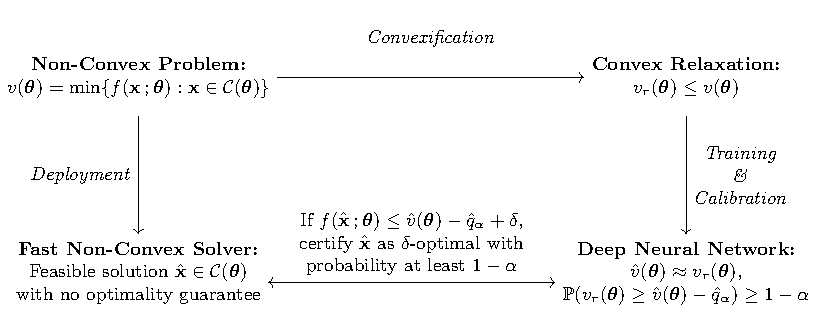
\includegraphics[width=0.85\linewidth]{figures/framework_diagram.pdf}
    \vspace{.05in}
    \caption{Our proposed approach for neural network-based optimality certification.}
    \label{fig:diagram}
\end{figure}
\section{Our Framework} \label{sec:approach}

We propose a framework which uses deep neural networks to certify global optima in non-convex optimization problems. We train a deep neural network $\hat{v}(\bm{\theta})$ to approximate the relaxed optimal value function $v_r(\bm{\theta})$ (the optimal value function of a convex relaxation) of a parametric non-convex problem. Given a new parameter instance $\bm{\theta} \in \Theta$, the neural network prediction $\hat{v}(\bm{\theta})$ may be compared with the objective value of any feasible solution $\hat{\mathbf{x}} \in \mathcal{C}(\bm{\theta})$ to estimate its optimality gap and thus certify whether $\hat{\mathbf{x}}$ is in fact near-globally optimal. 
We use convexification methods to trade off the tightness of convex relaxations with the computational cost of obtaining training data for the neural network. 
Furthermore, we use split conformal calibration to provide probabilistic guarantees on the accuracy of our optimality certificates.
We envision that our framework should supplement fast, approximate solvers, including local search methods, heuristic algorithms, and machine learning-based solvers, by providing probabilistic optimality certificates in online settings.

Our framework is based on a well-known strategy for certifying global optima using convexification methods.
For instance, \citet{xu2021verifying} propose to evaluate the KKT conditions of Lasserre hierarchy SDP relaxations at the candidate solution. Since the KKT conditions are sufficient to prove optimality in convex optimization, the candidate solution must be globally optimal if it satisfies the KKT conditions of the relaxed problem \citep{boyd2004convex}.
It also suffices to compare the optimal value of a convex relaxation with the objective value of the candidate solution.
Solving a convex relaxation provides a lower bound on the otherwise intractable optimal value $v_r(\bm{\theta}) \leq v(\bm{\theta})$ for any $\bm{\theta} \in \Theta$. The objective value of a candidate solution $\hat{\mathbf{x}} \in \mathcal{C}(\bm{\theta})$ may thus be compared against $v_r(\bm{\theta})$ to upper bound its \textit{optimality gap}, i.e. the gap between the solution's objective value and the optimal value:
\begin{align*}
    \text{\textit{optimality gap}} ~:=~ f(\hat{\mathbf{x}}\, ; \bm{\theta}) - v(\bm{\theta}) ~\leq~ f(\hat{\mathbf{x}}\, ; \bm{\theta}) - v_r(\bm{\theta}).
\end{align*}
Thus, if $f(\hat{\mathbf{x}}\,;\bm{\theta}) - v_r(\bm{\theta}) \leq \delta$, then $f(\hat{\mathbf{x}}\,;\bm{\theta}) - v(\bm{\theta}) \leq \delta$, certifying that $\hat{\mathbf{x}}$ is $\delta$-optimal.

One obvious disadvantage of this strategy is that the tightness of the upper bound depends on the size of the \textit{relaxation gap} $:= v(\bm{\theta}) - v_r(\bm{\theta})$, i.e. the gap between the original and relaxed problems' optimal values. It is non-trivial to bound the relaxation gap for an arbitrary convex relaxation of a non-convex problem. However, it is possible to control the relaxation gap by increasing the order of the convex relaxation within some convexification hierarchy (e.g., by introducing new valid inequalities or cutting planes). However, this typically would increase the size of the relaxed problem, making it slower to solve. 
%In short, tighter convex relaxations provide more accurate certificates, but are slower to solve. 
This is a fundamental limitation of this strategy that prevents it from being useful in large-scale time-varying optimization settings.
Our proposed framework overcomes this challenge by shifting the computational burden of solving large convex relaxations to an offline machine learning setting.
The power of convexification methods may thus be distilled into deep neural networks whose predictions can certify global optima in real-time.

Our proposed framework has four main steps: (1) convexification, (2) training, (3) calibration, and (4) deployment. Convexification involves finding a suitable convex relaxation of a parametric non-convex problem. Training involves generating a training data set by solving many instances of the convex relaxation offline, and training a deep neural network to approximate the relaxed optimal value function. Calibration involves conformalizing the neural network's predictions to guarantee a user-specified coverage rate for the relaxed optimal value. Finally, deployment involves choosing a certification threshold below which candidate solutions will be certified as near-globally optimal.
We describe these steps in greater detail below.

% TRADEOFF PARAGRAPH
%This is a central tradeoff in our framework: tighter convex relaxations provide more accurate optimality certificates, but are computationally expensive to solve for generating training data; however, insufficient training data can worsen the neural network's approximation error, leading to less accurate optimality certificates.

% Main Points: \\
% * We propose a framework which uses deep neural networks to certify the global optimality of solutions to non-convex optimization problems. We train deep neural networks $\hat{v}(\bm{\theta})$ to approximate the relaxed optimal value function $v_r(\bm{\theta})$ (the optimal value function of a convex relaxation) of a parametric non-convex problem. Given a new parameter instance $\bm{\theta} \in \Theta$, the neural network prediction $\hat{v}(\bm{\theta})$ may be compared with the objective value of any feasible solution $\hat{\mathbf{x}} \in \mathcal{C}(\bm{\theta})$ to estimate its optimality gap and thus certify whether $\mathbf{x}$ is near-globally optimal.\\
% * We envision that our framework should supplement fast, approximate solvers, including machine learning-based solvers, to provide probabilistic optimality guarantees without compromising speed in online optimization settings.\\
% * The framework uses convexification hierarchies to trade off the tightness of optimal value lower bounds with the computational cost of obtaining training data for the neural network.
% * Furthermore, the framework uses split conformal calibration to provide probabilistic guarantees on the accuracy of our optimality certificates.\\
% * Our framework is based on a well-known strategy for certifying global optima in non-convex problems: solving a convex relaxation and comparing with the value function (or, sometimes, checking local optimality conditions in the relaxed problem; Josz, Molzahn, etc.).
% * This approach has a fundamental limitation which prevent its use in online settings: the tradeoff between the relaxation gap and speed.\\
% * Our proposed approach overcomes this challenge by shifting the computational burden of obtaining near-optimal solutions to an offline learning problem. The power of convexification techniques may thus be distilled into deep neural networks which can assist in online optimization settings.
% * We outline the main steps of our framework below.\\
% * (Framework outline)

%We propose this method as a certification meta-framework. It is distinct from a standalone solver in that it is not tied to a single convexification technique. Any convexification trick, valid inequality, or instance-specific lower bound methodology from the optimization literature can be applied within our framework. The main novelty is the mechanism that allows us to take any computationally expensive convex relaxation---whether exact or approximate---and convert it into a millisecond-scale verified proxy. This bridges the gap between high-dimensional convex geometry and real-time optimization and control.

%Figure~\ref{fig:diagram} depicts the resulting pipeline, which decomposes into four stages. The first two (convexification, training) are performed entirely \textit{offline} and may be as computationally expensive as needed; the last two (calibration, deployment) are what make the framework usable \textit{online}, at the cost of only a probabilistic (rather than deterministic) optimality guarantee.

\paragraph{1. Convexification} Given a non-convex optimization problem \cref{prob:nonconvex}{}{} with value function $v(\bm{\theta})$, we construct a convex relaxation \cref{prob:convex-relax}{}{} with relaxed value function $v_r(\bm{\theta}).$
By construction, $v_r(\bm{\theta}) \leq v(\bm{\theta})$ for all $\bm{\theta} \in \Theta$, i.e. solving the relaxation for any parameter instance yields a valid lower bound on the true optimal value, which is generally intractable.
Within a convexification hierarchy, the order $r$ of the relaxation governs a trade-off central to our framework: a higher-order relaxation is tighter (smaller relaxation gap $v(\bm{\theta}) - v_r(\bm{\theta})$) but slower to solve. Because the convexified problem is solved offline, we may choose the tightest relaxation that remains tractable at the scale of the training set, rather than the scale of real-time deployment.

\paragraph{2. Training} We sample $N$ parameter instances $\bm{\theta}_1, \ldots, \bm{\theta}_N$ from a probability distribution $\mathbb{P}(\cdot)$ over $\Theta$ and solve the convex relaxation once per instance to obtain training pairs $(\bm{\theta}_i, v_r(\bm{\theta}_i))$. A deep neural network $\hat{v}(\bm{\theta})$ is then trained to approximate the relaxed value function by minimizing empirical mean-squared error:
\begin{equation*}
    \min_{\hat{v}(\cdot)}~ \frac{1}{N} \sum_{i=1}^N \big(v_r(\bm{\theta}_i) - \hat{v}(\bm{\theta}_i)\big)^2
\end{equation*}
Unlike solvers that learn a mapping to an optimal solution $\mathbf{x}^*(\bm{\theta})$, the prediction target here is always a scalar, regardless of the dimension of the decision variable $\mathbf{x} \in \mathcal{X}$ or the number of constraints in $\mathcal{C}(\bm{\theta})$. This is one reason the value function tends to be an easier learning target in practice.

\paragraph{3. Calibration} A trained network $\hat{v}(\bm{\theta})$ approximates $v_r(\bm{\theta})$ but offers no guarantee on any individual instance. We close this gap with split conformal calibration: using predictions on a held-out, exchangeable calibration set, we compute the one-sided conformal offset $\hat{q}_\alpha$ that satisfies
\begin{align*}
    \mathbb{P} \big( \, v_r(\bm{\theta}) \geq \hat{v}(\bm{\theta}) - \hat{q}_\alpha \, \big) \geq 1 - \alpha
\end{align*} at a user-specified miscoverage level $\alpha \in (0, 1)$. The quantity $\hat{v}(\bm{\theta}) - \hat{q}_\alpha$ is then a calibrated, probabilistic lower bound on $v_r(\bm{\theta})$ that holds with probability at least $1 - \alpha$.

\paragraph{4. Deployment} At runtime, we are given a parameter instance $\bm{\theta}$ and a feasible candidate solution $\hat{\mathbf{x}} \in \mathcal{C}(\bm{\theta})$ produced by any fast solver (local search method, heuristic algorithm, machine learning-based solver, etc.) with no optimality guarantee of its own. Evaluating $\hat{v}(\bm{\theta})$ costs a single forward pass through the neural network, which is orders of magnitude faster than re-solving the convex relaxation. We certify $\hat{\mathbf{x}}$ as $\delta$-optimal, for a target optimality gap $\delta > 0$, whenever
\begin{equation*}
    f(\hat{\mathbf{x}}\, ; \bm{\theta}) ~\leq~ \hat{v}(\bm{\theta}) - \hat{q}_\alpha + \delta.
\end{equation*}
Because $\hat{v}(\bm{\theta}) - \hat{q}_\alpha \leq v_r(\bm{\theta}) \leq v(\bm{\theta})$ holds with probability at least $1 - \alpha$, this certificate controls the probability of falsely declaring a candidate solution $\delta$-optimal when its true optimality gap in fact exceeds $\delta$.
To see this, let us directly analyze the false positive rate (FPR) of the optimality certificate:
\begin{align*}
    \mathit{FPR} ~:=~ \mathbb{P} \big( \, f(\hat{\mathbf{x}}\, ; \bm{\theta}) - \hat{v}(\bm{\theta}) \leq \delta - \hat{q}_\alpha \,|\, f(\hat{\mathbf{x}}\, ; \bm{\theta}) - v(\bm{\theta}) > \delta \, \big).
\end{align*}
By adding and subtracting $v(\bm{\theta})$, we may re-write this as
\begin{align*}
    \mathbb{P} \big( \, f(\hat{\mathbf{x}}\, ; \bm{\theta}) - v(\bm{\theta}) + v(\bm{\theta}) - \hat{v}(\bm{\theta} \, \big) \leq \delta - \hat{q}_\alpha \,|\, f(\hat{\mathbf{x}}\, ; \bm{\theta}) - v(\bm{\theta}) > \delta \, \big)
    \leq \mathbb{P} \big( \, \delta + v(\bm{\theta}) - \hat{v}(\bm{\theta}) \leq \delta - \hat{q}_\alpha \, \big),
\end{align*}
which simplifies to $\mathbb{P}(\hat{v}(\bm{\theta}) - v(\bm{\theta}) \geq \hat{q}_\alpha)$. Since $v_r(\bm{\theta}) \leq v(\bm{\theta})$ for all $\theta \in \Theta$, we have
\begin{align*}
    \mathbb{P}\big( \, \hat{v}(\bm{\theta}) - v(\bm{\theta}) \geq \hat{q}_\alpha \, \big ) \leq \mathbb{P} \big( \, \hat{v}(\bm{\theta}) - v_r(\bm{\theta}) \geq \hat{q}_\alpha \, \big) \leq \alpha
\end{align*}
by construction of $\hat{q}_\alpha$, hence the FPR of the certificate is bounded above by the miscoverage rate $\alpha$.

We also note that there are potentially multiple combinations of miscoverage rate $\alpha$ and optimality gap $\delta$ that lead to the same certification threshold. We may certify $\hat{\mathbf{x}} \in \mathcal{C}(\bm{\theta})$ as $\delta$-optimal with probability at least $1 - \alpha$ if $f(\hat{\mathbf{x}}\, ; \bm{\theta}) \leq \hat{v}(\bm{\theta}) + \tau$ for any $\alpha$, $\delta$ satisfying $\tau = \delta - \hat{q}_\alpha$. This lead to the notion of a \textit{frontier} of probabilistic optimality certificates with the same cutoff but with varying levels of precision and accuracy.

% Similarly, the false negative rate (FNR) is controlled by the relaxation gap $v(\bm{\theta}) - v_r(\bm{\theta})$.
% \begin{align*}
%     \mathit{FNR} ~:=~ \mathbb{P} \big( \, f(\hat{\mathbf{x}}\, ; \bm{\theta}) - \hat{v}(\bm{\theta}) > \delta -  \hat{q}_\alpha \,|\, f(\hat{\mathbf{x}}\, ; \bm{\theta}) - v(\bm{\theta}) \leq \delta \, \big).
% \end{align*}
% By adding and subtracting $v(\bm{\theta})$, we may re-write this as
% \begin{align*}
%     \mathbb{P}\big( \, f(\hat{\mathbf{x}}\, ; \bm{\theta}) - v(\bm{\theta}) + v(\bm{\theta}) - \hat{v}(\bm{\theta}) > \delta - \hat{q}_\alpha \,|\, f(\hat{\mathbf{x}}\, ; \bm{\theta}) - v(\bm{\theta}) \leq \delta \, \big)
%     \leq \mathbb{P} \big( \, \delta + v(\bm{\theta}) - \hat{v}(\bm{\theta}) > \delta - \hat{q}_\alpha \, \big),
% \end{align*}
% which simplifies to $\mathbb{P}( \hat{v}(\bm{\theta}) - v(\bm{\theta}) < \hat{q}_\alpha )$. Adding and subtracting $v_r(\bm{\theta})$, we have
% \begin{align*}
%     \mathbb{P}\big( \, \hat{v}(\bm{\theta}) - v_r(\bm{\theta}) + v_r(\bm{\theta}) - v(\bm{\theta}) < \hat{q}_\alpha\, \big) = \mathbb{P}\big( \, \hat{v}(\bm{\theta}) - v_r(\bm{\theta}) < \hat{q}_\alpha + v(\bm{\theta}) - v_r(\bm{\theta}) \, \big).
% \end{align*}
% The tightest bound we may achieve with this analysis is when $v(\bm{\theta}) - v_r(\bm{\theta})$, i.e. when there is no relaxation gap. In this case, the FNR is again bo
% This shows that in order to control the FNR, we should reduce both $\hat{q}_\alpha$ and the relaxation gap $v(\bm{\theta}) - v_r(\bm{\theta})$. However, reducing $\hat{q}_\alpha$ will necessarily increase $\alpha$ and thus possibly increase the FPR. Therefore, to reduce the FNR without increasing the FPR, the only option is to reduce the relaxation gap, i.e. increase the tightness of the convex relaxation.

% \begin{align*}
%     \mathbb{P}(f(\hat{\mathbf{x}}\, ; \bm{\theta}) - v(\bm{\theta}) \leq \delta \,|\, f(\hat{\mathbf{x}}\, ; \bm{\theta}) - \hat{v}(\bm{\theta}) \leq \delta - \tau) \\
%     =~ \mathbb{P}(f(\hat{\mathbf{x}} \, ; \bm{\theta}) - \hat{v}(\bm{\theta}) + \hat{v}(\bm{\theta}) - v(\bm{\theta}) \leq \delta \,|\, f(\hat{\mathbf{x}}\, ; \bm{\theta}) - \hat{v}(\bm{\theta}) \leq \delta - \tau) \\
%     \geq~ \mathbb{P}(\delta - \tau + \hat{v}(\bm{\theta}) - v(\bm{\theta}) \leq \delta)\\ 
%     =~ \mathbb{P}(\hat{v}(\bm{\theta}) - v(\bm{\theta}) \leq \tau) \\
%     \geq~ \mathbb{P}(\hat{v}(\bm{\theta}) - v_r(\bm{\theta}) \leq \tau) \geq 1 - \alpha.
% \end{align*}

% Noooo... this doesn't work?

% Consider a parametric optimization problem:
% \vspace{-0.75em}
% \begin{equation}
% \begin{aligned}
%     v(p) := ~\min_{x \in \mathbb{R}^n}~~~&f(x;p)  \\
%     \text{s.t.}~~~~& g(x; p) \leq 0
% \end{aligned} \label{eq:parametric_opt}
% \vspace{-0.75em}
% \end{equation}
% in which the parameter $p \in \Phi \subseteq \mathbb{R}^d$ (where $\Phi$ is an arbitrary parameter set).
% We assume that \eqref{eq:parametric_opt} is feasible for all $p \in \Phi$. The value function $v: \mathbb{R}^d \to \mathbb{R}$ expresses the globally optimal objective value as a function of the parameter $p$. The objective function $f(x;p)$ and/or the constraints $g(x;p)$ may be non-convex, so \eqref{eq:parametric_opt} may be a non-convex problem.

% The value function may be used to test optimality of arbitrary feasible solutions. Given $\hat{x} \in \mathbb{R}^n$ that is feasible for \eqref{eq:parametric_opt}, if the cost $f(\hat{x};p) = v(p)$ then $\hat{x}$ is optimal; otherwise, if $f(\hat{x};p) > v(p)$, it is not.

% Furthermore, \textit{approximations} of the value function may be used to test \textit{near}-optimality of arbitrary feasible solutions. Let $\hat{v}(p)$ be a function that approximates $v(p)$ over $\Phi$. If one can bound the approximation error of $\hat{v}(p)$ over $\Phi$, then they may also bound the optimality gap $f(\hat{x};p) - v(p)$ by comparing $f(\hat{x};p)$ to $\hat{v}(p)$. 

% These observations motivate our work in this paper: we propose a machine learning framework to approximate the value functions of non-convex optimization problems for the purpose of approximate optimality certification. This framework may be especially beneficial in online settings, where obtaining exact optimality certificates may be expensive or impractical.

% In particular, we propose to train a neural network to approximate $v(p)$ over the parameter set $\Phi$. 
% We solve many instances of \eqref{eq:parametric_opt} for different $p \in \Phi$ to get training samples $(p_i, v(p_i))$ with $i$ ranging from $1$ to $N$.
% The neural network $\hat{v}_{\theta}(p)$ is trained to minimize the mean-squared error loss:
% \vspace{-0.5em}
% \setlength{\jot}{0pt}
% \begin{align}
%     \min_\theta~ \frac{1}{N} \sum_{i=1}^{N} (v(p_i) - \hat{v}_{\theta}(p_i))^2
%     \label{eq:learning-problem}
% \end{align}
% where $\theta$ represents the network's weights and biases.
% If the trained neural network $\hat{v}_\theta(p)$ achieves low approximation error over the full parameter set $\Phi$, we may use it to certify near-optimality of solutions obtained via local search methods or other solvers. (Hereafter, we drop the `$\theta$' subscript notation for $\hat{v}(p)$ when referring to trained neural networks.)

% The central challenge of learning to approximate the value function is developing a rich training data set. This is because evaluating $v(p)$ many times may be expensive, as it involves repeatedly solving a non-convex optimization problem.
% This challenge may not always be easily overcome. However, for a large class of non-convex problems, convexification techniques allow us to find globally optimal solutions relatively efficiently. Therefore, the use of convexification techniques is a key element of our framework.

% We now describe the role of convexification techniques within our framework. Consider a convex relaxation of problem \eqref{eq:parametric_opt}:
% \begin{equation}
% \begin{aligned}
%     \tilde{v}(p) := ~\min_{x \in \mathbb{R}^n,~ u \in \mathbb{R}^k}~&\tilde{f}(x, u;p)  \\
%     \text{s.t.}~~~~~& \tilde{g}(x, u; p) \leq 0
% \end{aligned} \label{eq:convex_parametric_opt}
% \end{equation}
% where $\tilde{f}(x,u;p)$ and $\tilde{g}(x, u; p)$ are convex outer-approximations of $f(x;p)$ and $g(x; p)$, respectively, and $u \in \mathbb{R}^k$ are (optional) additional variables introduced to lift or convexify the problem.
% Hereafter, we use $\tilde{v}(p)$ to denote the value function of any convex relaxation. Since \eqref{eq:convex_parametric_opt} is a convex relaxation of \eqref{eq:parametric_opt}, we have that $\tilde{v}(p) \leq v(p)$ for all $p \in \Phi$. Therefore, solving \eqref{eq:convex_parametric_opt} always yields a global lower bound on $v(p)$. When $\tilde{v}(p) = v(p)$, we say the relaxation is ``exact."

% One may evaluate $v(p)$ in polynomial time by solving an \textit{exact} convex relaxation of \eqref{eq:parametric_opt}. This key insight enables our framework to be applied to any non-convex problem for which an exact or tight convex relaxation exists. By finding an exact convex relaxation of \eqref{eq:parametric_opt} for (almost) any $p \in \Phi$, one may solve problem instances of \eqref{eq:parametric_opt} relatively efficiently to develop a training data set for the learning problem \eqref{eq:learning-problem}.

% %The tightest possible convex relaxation of \eqref{eq:epigraph_reformulation} is obtained by taking $\tilde{\mathcal{F}}(p) = \text{conv}(\mathcal{F}(p))$, i.e. the convex hull of $\mathcal{F}(p)$. However, this set is not easy to construct in general. Indeed, constructing the convex hull of $\mathcal{F}(p)$ may be just as hard as solving the original non-convex problem. 

% As an important caveat, we note that convexification enables exact evaluation of $v(p)$ at the potential expense of slower computation due to the much larger size of the convexified problem.
% This is precisely why we propose to use convexification techniques \textit{offline} to develop training data sets, and use neural networks \textit{online} to provide approximate optimality certificates.

% \subsection{Convexification Techniques}

% Convexification is a powerful approach for globally solving non-convex problems. The basic idea of convexification is to replace non-convex objectives or constraints with convex outer-approximations. The resulting convex problem is a relaxation of the original non-convex problem, and may be solved in polynomial time. The optimal value of the convex relaxation is a lower bound on the optimal value of the original problem. In some cases, an optimal solution of the original problem may be recovered from the convex relaxation, meaning the original problem may also be solved in polynomial time.

% % Convexification has been used to tackle non-convex problems in a variety of domains. In combinatorial optimization, \citet{goemans1995improved} famously used semidefinite relaxation and randomization techniques to develop an approximate solution algorithm for the max-cut problem. \citet{sherali1990hierarchy} introduce a linear programming (LP) hierarchy to approximate the convex hull of 0-1 programming problems in higher dimensional spaces.
% % \citet{bienstock2008approximate} constructs an approximate extended linear formulation of the 0-1 knapsack problem with a polynomial number of variables and constraints.
% % The Lasserre hierarchy constructs a sequence of increasingly tight semidefinite relaxations of polynomial optimization problems \cite{lasserre2001global}. \citet{sojoudi2014exactness} provide sufficient conditions for the exactness of semidefinite and second-order cone relaxations of a large class of non-linear optimization problems. 
% % In power systems, \cite{lavaei2012zero} propose a semidefinite relaxation of AC-OPF and provide sufficient conditions for exactness (see \citet{low2014convex} for a review of convex relaxations of AC-OPF). \citet{molzahn2016moment} study higher order semidefinite relaxations of AC-OPF, which are generally tighter but much larger and slower to solve. 

% % Indeed, a common theme among convexification methods is that convexified problems may be orders of magnitude larger than the original non-convex problem, making these techniques cumbersome to use in online settings. 
% % %For instance, to approximate the 0-1 knapsack polytope with $n$ items to within a factor of $\epsilon$, Bienstock (2004)'s extended linear formulation would require $\mathcal{O}(\epsilon^{-1}n^{1+\lceil 1/\epsilon \rceil})$ variables and $\mathcal{O}(\epsilon^{-1}n^{2+\lceil 1/\epsilon \rceil})$ constraints.
% % For instance, for 0-1 programming problems in $\mathbb{R}^n$, the order-$d$ Sherali-Adams hierarchy LP has $\sum_{i=1}^{d}\binom{n}{i}$ variables.
% % The SDP relaxation of a QCQP has $n(n+1)/2$ variables compared to $n$ variables in the original problem.
% % For an arbitrary polynomial optimization problem in $\mathbb{R}^n$, the decision variable of the order-$d$ Lasserre hierarchy SDP is a $\binom{n+d}{d} \times \binom{n+d}{d}$ symmetric positive semidefinite matrix. High-order SDPs of the Lasserre hierarchy quickly become impractical to solve in real-time for even moderate-sized polynomial optimization problems. However, we claim that the power of convexification may be harnessed to \textit{learn} the value function of a non-convex problem \textit{offline} and thus provide optimality certificates.


% \subsubsection{Structured QCQP} \label{sec:structured-QCQP}

% Our method is highly compatible with structured QCQP, which is a class of QCQPs that exhibit specific structure -- either in the objective, the constraints, or both -- that can be exploited to make the problem easier to solve or analyze.

% Many non-convex problems, including integer programming problems, may be exactly or approximately represented as polynomial optimization problems (POPs). A generic POP can be written as
% \begin{equation}
% \begin{aligned}
% \min_{x \in \mathbb{R}^n}~& f(x) = \sum_\alpha f_\alpha x^\alpha \\
% \text{s.t.}~~& g_i(x) =\sum_\alpha g_{i, \alpha} x^\alpha \geq 0, \quad i=1, \ldots, m
% \end{aligned}
% \label{eq:POP}
% \end{equation}
% where both the objective \( f(x) \) and constraints \( g_i(x) \) are polynomials in \( x \in \mathbb{R}^n \). We use the multi-index notation $x^\alpha:=x_1^{\alpha_1} \cdots x_n^{\alpha_n}$ for $x \in \mathbb{R}^n$ and $\alpha \in \mathbb{N}^n$.

% Furthermore, a generic POP may be re-formulated via quadrification \citep{sherali2013reformulation, dalkiran2018linear} as a QCQP of the form
% \begin{equation}
% \begin{aligned}
%     \min_{y \in \mathbb{R}^k}~& y^T M_0 y \\
%     \text{s.t.}~& y^T M_i y \geq 0, \quad i = 1, 2, ..., l.
% \end{aligned}
% \label{eq:QCQP}
% \end{equation}
% Generally, this requires introducing new variables and constraints to re-write higher degree ($> 2$) monomials as quadratic terms. For example, the constraint `$3x^6 - 2x^2 \geq 0$' may be equivalently represented by the constraints `$y = x^2$, $~z = y^2$, and $3yz - 2y \geq 0$.'
% As a result, the equivalent QCQP may be much larger than the original POP in terms of the number of variables ($k \gg n$) and constraints ($l \gg m$). 

% Non-convex QCQPs are therefore a very broad class of optimization problem. Importantly, their simple structure has allowed for detailed study of QCQP convexification. In particular, a number of structural characterizations have been developed which are sufficient for exactness of the SDP relaxation of a QCQP:
% \begin{equation}
% \begin{aligned}
%     \min_{Y \in \mathbb{R}^{n \times n}}~& \langle M_0, Y \rangle \\
%     \text{s.t.}~~~& \langle M_i, Y\rangle \geq 0, \quad i = 1, 2, ..., l\\
%     &~~ Y \succeq 0
% \end{aligned}
% \label{eq:SDP_relaxation}
% \end{equation}
% Examples of such structural characterizations include conditions on the number of constraints in \eqref{eq:QCQP}, such as the $S$-lemma \citep{boyd2004convex} and a number of more general results on low-rank SDP relaxations \citep{lemon2016low}. For example, the $S$-lemma proves the exactness of an SDP relaxation of a QCQP with a single quadratic constraint. Other examples include conditions on the underlying graph structure of the QCQP, as in \citet{sojoudi2014exactness} and \citet{bose2015quadratically}. For instance, if the underlying graph of a QCQP is acyclic, then its SDP relaxation must be exact. QCQPs with exact SDP relaxations may be solved efficiently, even if they have disconnected feasible regions or multiple local minima.

% Additionally, exactness of the SDP relaxation of a QCQP may be ascertained not only \textit{a priori} via structural characterizations but also \textit{a posteriori} by proving feasibility of the optimal solution in the original problem. 
% For example, exactness may ascertained from the rank of an optimal solution \citep{lemon2016low}. If $Y^*$ is optimal for the SDP relaxation \eqref{eq:SDP_relaxation} and $\text{rank}(Y^*) = 1$, then there exists a vector $x^* \in \mathbb{R}^n$ such that $Y^* = y^* y^{*T}$ and that is feasible (and thus optimal) for \eqref{eq:QCQP}. Therefore, whenever \eqref{eq:SDP_relaxation} is an exact relaxation of \eqref{eq:QCQP}, the minimum values of the two problems coincide and a globally optimal solution of \eqref{eq:QCQP} may be recovered from a solution of \eqref{eq:SDP_relaxation}. If there are multiple optimal solutions to \eqref{eq:SDP_relaxation}, it is possible that an optimal solution $Y^*$ obtained from an SDP solver is not rank-1 even though a rank-1 solution exists, in which case the optimal values agree anyways.

% \subsubsection{QCQPs with Convex Value Functions}

% Consider a QCQP parameterized by right-hand side uncertainty:
% \begin{align}
%     v(b) := \min_{y \in \mathbb{R}^k}~& y^T M_0 y \label{eq:QCQP_parametric} \\
%     \text{s.t.}~& y^T M_i y \geq b_i, \quad i = 1, 2, ..., l \nonumber
% \end{align}
% As a minor point, we observe that if the parametric QCQP \eqref{eq:QCQP_parametric} admits an exact convex relaxation for all parameters $b \in \Phi$ where $\Phi \subseteq \mathbb{R}^m$ is some convex parameter set, then the value function $v(b)$ is convex over $\Phi$. The proof of this statement is trivial and follows the well-known argument for convexity of the value function of convex problems parameterized by right-hand side uncertainty.  However, the result is useful in practice. For instance, load-parameterized AC-OPF falls into this category of parametric QCQPs. The result also has implications for the \textit{types} of neural networks that can approximate the value functions of QCQPs.
% \subsubsection{Sum-of-Squares and Lasserre Hierarchy}
% Testing whether a polynomial \( f(x) \) is globally non-negative (\( f(x) \geq 0, \forall x \)) is NP-hard~\citep{murty1985some}. However, the sum of squares (SOS) decomposition provides a sufficient condition for non-negativity~\citep{parrilo2003semidefinite}. A polynomial \( p(x) \) is an SOS if there exist polynomials \( q_i(x) \) such that $p(x) = \sum_{i=1}^m q_i^2(x)$. 

% Let $\Sigma[x]$ be the set of SOS polynomials, which forms a convex cone, and $\Sigma[x]_d$ be the set of SOS polynomials of degree at most $2 d$. A polynomial $\sigma(x) \in \Sigma_d[x]$ if it is of the form
% \vspace{-1em}
% \begin{equation}
% \label{eq:SOS-d-def}
% \sigma(x)=\sum_k\left(\sum_{|\alpha| \leqslant d} p_{k, \alpha} x^\alpha\right)^2 \text { where } p_{k, \alpha} \in \mathbb{R}.
% \end{equation}
% This is equivalent to the existence of $\left(\varphi_{\alpha, \beta}\right)_{|\alpha|,|\beta| \leqslant d} \succcurlyeq 0$ such that $\sum_{|\alpha| \leqslant 2 d} \sigma_\alpha x^\alpha=\sum_{|\alpha|,|\beta| \leqslant d} \varphi_{\alpha, \beta} x^{\alpha+\beta}$.
% %(note that $\succcurlyeq$ is the positive semidefinite sign). 

% Let $\mathbf{S}:=\left\{x \in \mathbb{R}^n \mid g_1(x) \geq 0, \ldots, g_m(x) \geq 0\right\}$, $\mathscr{M}(\mathbf{S})$ be the vector space of finite signed Borel measures supported on $\mathbf{S}$, and $\mathscr{M}_{+}(\mathbf{S})$ denote the cone of nonnegative elements of $\mathscr{M}(\mathbf{S})$. Problem~\eqref{eq:POP} can be reformulated as a linear program over probability measures~\citep{lasserre2015introduction}:

% \begin{equation}
% \min _{\mu \in \mathscr{M}_{+}(\mathbf{S})}\left\{\int_{\mathbf{S}} f \mathrm{~d} \mu: \int_S \mathrm{~d} \mu=1\right\}.
% \label{eq:pop-measure}
% \end{equation}

% To make this reformulation tractable, we introduce the $r$-th order moment matrix $\mathbf{M}_r(y)$ associated with a sequence $y$, and the $r$-th order localizing matrix $\mathbf{M}_{r}\left(g_j y\right)$ associated with $y$ and constraint $g_j$:
% \vspace{-0.5em}
% \begin{equation}
% \begin{aligned}
% \mathbf{M}_r(y)&\coloneq\left(y_{\alpha+\beta}\right)_{|\alpha|,|\beta| \leqslant r}\\
% \mathbf{M}_{r}\left(g_j y\right)&\coloneq(\sum_\gamma g_{i, \gamma} y_{\alpha+\beta+\gamma})_{|\alpha|,|\beta| \leqslant r}
% \end{aligned}
% \label{eq:Mr-def}
% \vspace{-0.5em}
% \end{equation}
% We construct a hierarchy of moment relaxations for problem~\eqref{eq:pop-measure}, as $\mu \in \mathscr{M}_{+}(\mathbf{S})$ can be relaxed to $\mathbf{M}_{r-d_j}\left(g_j y\right) \succeq 0$, for all $j=0, \ldots, m$, and all $r \geq d_j=\left\lceil\operatorname{deg}\left(g_j\right) / 2\right\rceil$. Here, $\lceil\cdot\rceil$ denotes the ceiling function, and $\operatorname{deg}(\cdot)$ denotes the degree of a polynomial function.

% Letting $r_{\min }\coloneq\max \left\{\lceil\operatorname{deg}(f) / 2\rceil, d_1, \ldots, d_m\right\}$, for $r \geq r_{\text {min }}$ of the hierarchy, we construct the order-$r$ moment SDP:
% \begin{equation}
% \begin{aligned}
% \min _{y}\quad & L_{y}(f)  \\
% \text { s.t. }\ \ \ &
% \mathbf{M}_r(y) \succeq 0 \\
% &  \mathbf{M}_{r-d_j}\left(g_j y\right) \succeq 0, \quad j =1,\dots,m \\
% & y_0=1
% \end{aligned}
% \label{eq:pop-relax}
% \end{equation}

% \vspace{-1em}
% where $L_{y}(f)\coloneq \sum_\alpha f_\alpha y^\alpha$, and $y \in \mathbb{R}^{\frac{(n+2r)\dots (n+1)}{(2r)!}}$. The dual of problem~\eqref{eq:pop-relax} is thus the following optimization problem over SOS polynomials of order $r$:
% \vspace{-0.5em}
% \begin{equation}
% \label{eq:Lasserre-sos}
% \begin{array}{cc}
% \underset{\lambda, \sigma}\max & \lambda \\
% \text { s.t. } & f-\lambda=\sigma_0+\sum_{k=1}^m \sigma_k g_k \\
% & \lambda \in \mathbb{R}, \sigma_0 \in \Sigma_r[x], \\
% & \sigma_i \in \Sigma_{r-d_j}[x], \quad j=1, \ldots, m .
% \end{array}
% \end{equation}
% The Lasserre hierarchy, presented here, thus provides a sequence of SDP relaxations for solving the POP \eqref{eq:POP}. By defining $\mathcal{M}(\mathfrak{g})$ to be the quadratic module generated by $\mathfrak{g}$,  the following theorem provides a powerful condition for $\lambda$ to be a  lower bound on $f$.

% \begin{theorem}[Putinar's Positivstellensatz~\citep{putinar1993positive}]
% Assume that there exists $N>0$ such that $N-\|x\|_2^2 \in \mathcal{M}(\mathfrak{g})$ (Archimedean's condition). If $f$ is positive on $\mathbf{S}$, then
% \vspace{-0.5em}
% \begin{equation}
% \label{eq:thm-sos}
% f=\sigma_0+\sigma_1 g_1+\cdots+\sigma_m g_m,
% \end{equation}
% where $\sigma_0, \ldots, \sigma_m$ are SOS.
% \vspace{-0.5em}
% \end{theorem} 
% Under the Archimedean condition, the hierarchy converges to the global optimum of the original problem as $r \to \infty$~\citep{lasserre2001global}. Importantly, the relaxation error is asymptotically bounded by $\mathcal{O}(1/r)$. For specific problem classes, such as those with a ball constraint, there is often no duality gap even at lower relaxation levels~\citep{josz2016strong}. In cases where basic relaxations ($r=1$) are insufficient or inexact, our framework naturally incorporates higher levels of the Lasserre hierarchy to tighten the bounds.

% This flexibility allows for a strategic trade-off: one may choose a higher-order relaxation ($r \ge 2$) to reduce the relaxation gap $v(p) - \tilde{v}(p)$ and improve certificate quality, at the expense of increased offline computational cost for data generation. For instance, \citet{molzahn2016moment} demonstrate that while second-order relaxations for AC-OPF are tighter than first-order ones, they are significantly more expensive to solve. Our framework is agnostic to the chosen hierarchy level: it simply learns the value function $\tilde{v}(p)$ of a particular relaxation, which still provides a lower bound on $v(p)$ even when the relaxation is not exact.

\begin{figure}[ht!]
    \centering
    \begin{minipage}[t]{0.49\textwidth}
        \centering
        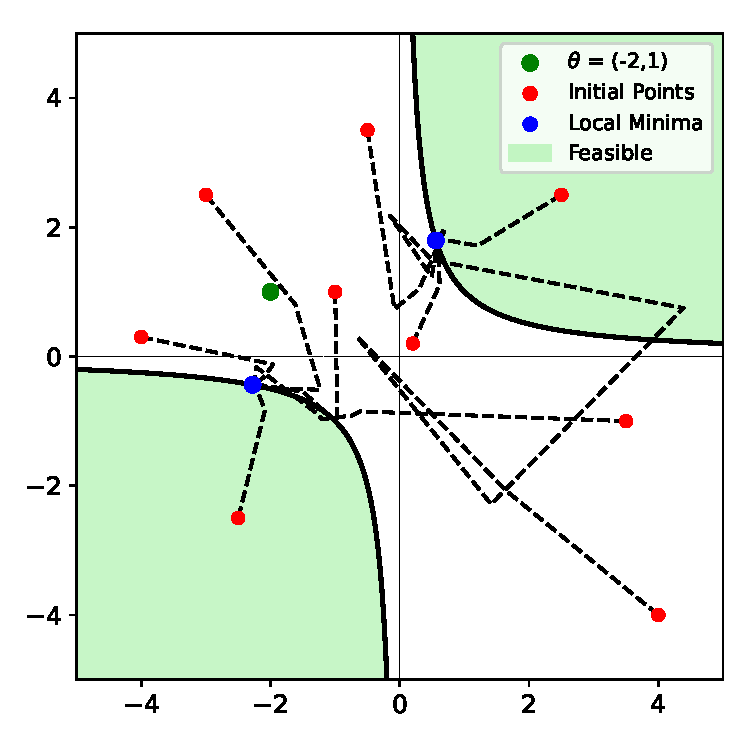
\includegraphics[width=\linewidth]{figures/QCQP_example_convergence.pdf}
        \caption{Interior point method convergence behavior for problem \cref{prob:qcqp}{}{} for $\bm{\theta} = (-2,1)$. 
        %The global minimum is near $(-2.3, -0.5)$, but a spurious local minimum is near $(0.6, 1.8)$.
        }
        \label{fig:QCQP_example_fig}
    \end{minipage}
    \vspace{-0.5em}
    \hfill
    \begin{minipage}[t]{0.49\textwidth}
        \centering
        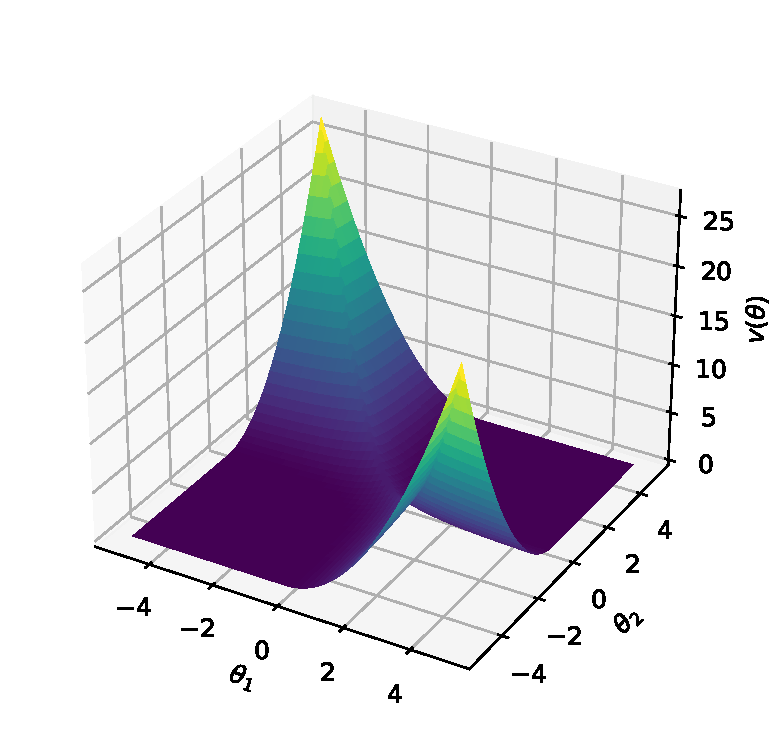
\includegraphics[width=\linewidth, trim=0 0 40 0]{figures/3d_value_function_plot.pdf}
        \caption{Optimal value function $v(\bm{\theta})$ over the parameter space $\Theta = [-5, 5] \times [-5, 5]$ for problem \cref{prob:qcqp}{}{}.}
        \label{fig:QCQP_vhat_fig}
    \end{minipage}
    \vspace{-0.5em}
\end{figure}

\subsection{Example Problem: QCQP} \label{subsec:illustrative_example}

Let us illustrate our framework in a simple problem setting.
Consider the following parametric quadratically-constrained quadratic program (QCQP) over $x \in \mathbb{R}^2$:
\setlength{\jot}{2pt}
\begin{equation}
\begin{aligned}
    v(\bm{\theta}) ~=~ \min_{x \in \mathbb{R}^2} \quad &(x_1 - \theta_1)^2 + (x_2 - \theta_2)^2 \\
    \text{s.t.}\quad& x_1 x_2 \geq 1
\end{aligned}
\label{prob:qcqp}
\end{equation}

In words, the problem is to find a point of minimum squared distance to $\bm{\theta} \in \mathbb{R}^2$ satisfying $x_1 x_2 \geq 1$. The quadratic constraint yields a non-convex feasible set with two disconnected regions. Therefore, any instance of this problem has two local minima.

As illustrated in Figure \ref{fig:QCQP_example_fig}, the convergence behavior of local search methods depends strongly on the initial point used in the search. Some initial points converge to the global minimum while others converge to the spurious local minimum. A naive strategy would be to try multiple initial points and keep the best solution found. However, without a principled strategy for selecting initial points (or problem-specific knowledge about the number of local minima), it is not clear when to terminate this procedure. We now illustrate our framework's ability to certify global optima in this problem.

\paragraph{1. Convexification} We shall convexify problem \cref{prob:qcqp} via semidefinite relaxation. We lift the problem to the space of symmetric positive semidefinite (PSD) matrices. Entries of the lifted matrix variable $Y \in \mathbb{S}^{3 \times 3}$ replace monomials in the objective and constraints of the original problem. For example, $Y_{11}$ replaces $x_1^0 x_2^0 = 1$, $Y_{22}$ replaces $x_1^2 x_2^0 = x_1^2$, and $Y_{23}$ replaces $x_1^1 x_2^1 = x_1 x_2$. The semidefinite relaxation of problem \cref{prob:qcqp} is therefore
\begin{equation}
\begin{aligned}
v_r(\bm{\theta}) ~=~ \min_{Y \in \mathbb{S}^{3 \times 3}} \quad 
&Y_{22} + Y_{33} - 2 \theta_1 Y_{12} - 2 \theta_2 Y_{13} + (\theta_1^2 + \theta_2^2) Y_{11} \\ 
\text{s.t.}\quad & Y_{11} = 1 \\[3pt]
& Y_{23} \geq 1 \\[4pt]
& ~Y \succeq 0
\end{aligned}
\label{prob:qcqp_relaxed}
\end{equation}
The relaxation \cref{prob:qcqp_relaxed} is always exact, i.e. $v_r(\bm{\theta}) = v(\bm{\theta})$ for all $\bm{\theta} \in \mathbb{R}^2$, because problem \cref{prob:qcqp}{}{} has only one quadratic inequality constraint (see $S$-lemma; \cite{boyd2004convex}). 
%Because the relaxation gap is zero everywhere, the error in our experiments is entirely attributable to the neural network's approximation error.

\paragraph{2. Training} We sample $20{,}000$ training instances and $5{,}000$ test instances of $\bm{\theta}$ uniformly at random over $\Theta = [-5,5] \times [-5,5]$. We compute the relaxed optimal value $v_r(\bm{\theta})$ for each instance by solving problem \cref{prob:qcqp_relaxed}{}{}. We then train deep neural networks $\hat{v}(\bm{\theta})$ to approximate $v_r(\bm{\theta})$ via four-fold cross-validation (see Section \ref{sec:experiments} for a detailed description of our neural network training procedure). The trained neural network achieves a mean absolute error (MAE) of $0.0022$ over the test data set.

\paragraph{3. Calibration} For each fold, we compute the upper $\alpha$-quantile of the held-out set prediction errors, $\hat{q}_\alpha = 0.012$, for a chosen miscoverage rate of $\alpha = 1\%$, which we use to conformalize the neural network's predictions in the deployment phase to control the false positive rate.

\paragraph{4. Deployment} We solve each problem instance in the test set with IPOPT, a local interior point solver, from a random fixed initialization \citep{wachter2006implementation}. For each feasible local solution $\hat{\mathbf{x}}$ obtained by the local solver, we certify optimality if $f(\hat{\mathbf{x}}\,;\bm{\theta}) \leq \hat{v}(\bm{\theta}) + \delta - \hat{q}_\alpha$ for a chosen optimality tolerance $\delta = 0.138$. The optimality tolerance is calibrated to be $3 \% \times \text{std.\,} v(\bm{\theta})$, so that we may certify optimality within $3\%$ of the intrinsic variability of $v(\bm{\theta})$. The certification threshold is therefore $\delta - \hat{q}_\alpha = 0.126$. The neural network is extremely accurate relative to this certification threshold, and achieves zero false positive rate and near-zero false negative rate for certifying global optima over the test data set (results in \cref{tab:combined}{}{}).

\section{Experiments} \label{sec:experiments}

We evaluate our framework on four parametric non-convex problems drawn from robotics, power systems, digital communications, and integer programming.

\subsection*{Experimental Procedure}

Each experiment instantiates the framework of Section~\ref{sec:approach}. We fix a convex relaxation of the problem and generate training data by randomly sampling 
$20{,}000$ training and $5{,}000$ test parameters $\bm{\theta}_i \in \Theta$ and solving the relaxation for each to obtain $(\bm{\theta}_i, v_r(\bm{\theta}_i))$. 
We then train a four-fold ensemble of deep networks $\hat{v}(\bm{\theta})$ to approximate the relaxed value function $v_r(\bm{\theta})$ (Section~\ref{subsec:dnn}) and calibrate each fold on its own held-out partition. Every test parameter is additionally solved by a fast local or heuristic solver to obtain the feasible solution $\hat{\mathbf{x}}(\bm{\theta})$ that the framework then certifies. We vary these ingredients across experiments, comparing convex relaxations of different orders (first- vs.\ second-order Lasserre SDP relaxation for inverse kinematics, SOCP vs.\ chordal SDP for AC-OPF), different fast solvers, different training sizes, and studying problem scales spanning three orders of magnitude.

We deploy the certificate of Section~\ref{sec:approach} (certifying $\hat{\mathbf{x}}$ as $\delta$-optimal when $f(\hat{\mathbf{x}}\,;\bm{\theta}) \leq \hat{v}(\bm{\theta}) - \hat{q}_\alpha + \delta$) at a single fixed operating point throughout,
\begin{equation*}
    \delta \,=\, 3 \% \times \mathrm{std.\,}v(\bm{\theta}), \qquad \alpha \,=\, 0.01,
\end{equation*}
so that a certified solution is within $3\%$ of the intrinsic variability of the optimal value $v(\bm{\theta})$ across instances, with $99\%$ confidence (conformal offset $\hat{q}_{99}$). Scaling $\delta$ to the optimal value spread rather than a fixed relative optimality gap keeps the tolerance meaningful across problems of vastly different magnitude and avoids instability the instability of relative gaps when the optimal value is near zero. We score each certificate against the ground-truth event $f(\hat{\mathbf{x}}\,;\bm{\theta}) - v(\bm{\theta}) \leq \delta$, using the exact optimal value $v(\bm{\theta})$ where tractable and the relaxed optimal value $v_r(\bm{\theta})$ otherwise, and report true/false positive/negative counts (TP, FP, TN, FN) averaged over the four folds to demonstrate the accuracy of our framework in each problem setting.

\subsection*{Deep Neural Networks} \label{subsec:dnn}

Across all experiments we use a single network architecture and training recipe, selected by an ablation study on the AC-OPF problem (Appendix~\ref{app:ablation}). The network is a fully-connected feedforward network with six hidden layers of $256$ ReLU units each, mapping the parameter $\bm{\theta}$ to a scalar value function estimate $\hat{v}(\bm{\theta})$. Network inputs and the regression target are standardized to zero mean and unit variance using statistics computed on the training partition, and predictions are mapped back to physical units at inference.

We train for $1000$ epochs with the AdamW optimizer (learning rate $10^{-3}$, weight decay $10^{-4}$, batch size $256$) under a cosine-annealed learning-rate schedule. We partition the $20{,}000$ training samples with $4$-fold cross-validation (a fixed random shuffle, held constant across all experiments so that the split is reproducible), training one model per fold. Each fold's heldout validation partition serves as the conformal calibration set for that fold model, per step~(4) above. A representative training history is shown in Figure~\ref{fig:training-history}: both the training and validation loss decay by roughly five orders of magnitude and track one another closely throughout training, indicating that the network fits the value function without overfitting.

\begin{figure}[t]
    \centering
    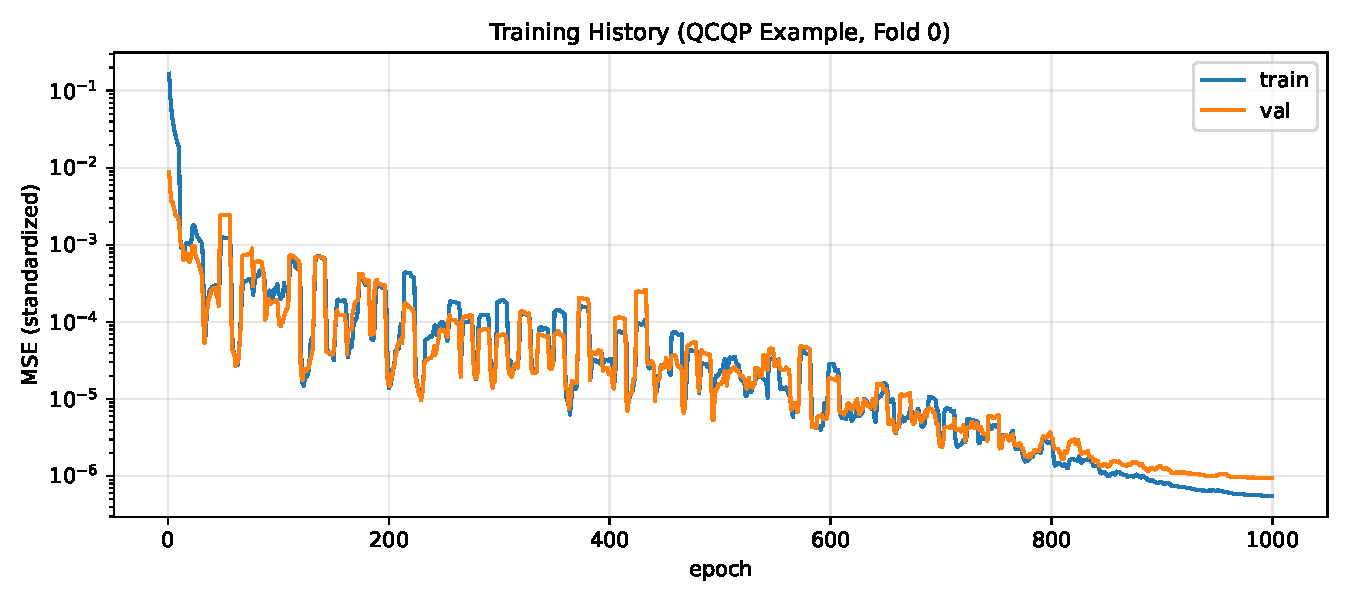
\includegraphics[width=\linewidth]{figures/fig_training_history.pdf}
    \caption{Training and validation loss (mean-squared error on the standardized target) for a representative fold model, on a logarithmic scale. The loss decays smoothly under the cosine-annealed schedule, with training and validation curves tracking closely.}
    \label{fig:training-history}
\end{figure}

\subsection{Robotics: Inverse Kinematics} \label{subsec:IK}

Inverse kinematics is a fundamental problem in robotics: given a target position for a robot's end effector, one must recover joint configurations that place the end effector at or as near as possible to the target. We consider a two-link planar arm with link lengths $\ell_1, \ell_2$ and joint angles $\phi_1, \phi_2$, parameterized by a target position $\bm{\theta} \in \mathbb{R}^2$.
We reformulate this problem as a QCQP by lifting via trigonometric identities.
Letting $c_i = \cos\phi_i$ and $s_i = \sin\phi_i$ for $i \in \{1, 2\}$, the end effector position is $(x_1, x_2) = \big(\ell_1 c_1 + \ell_2 c_{12},~ \ell_1 s_1 + \ell_2 s_{12}\big)$, where $c_{12} = c_1 c_2 - s_1 s_2$ and $s_{12} = s_1 c_2 + c_1 s_2$ by trigonometric identities. The problem of minimizing squared distance to the target is therefore the non-convex QCQP
\begin{equation}
\begin{aligned}
    v(\bm{\theta}) ~=~ \min_{(c, s) \in \mathbb{R}^4} \quad & (x_1 - \theta_1)^2 + (x_2 - \theta_2)^2 \\
    \text{s.t.} \quad & c_1^2 + s_1^2 = 1 \\
    & c_2^2 + s_2^2 = 1 \\
    & x_1 = \ell_1 c_1 + \ell_2 (c_1 c_2 - s_1 s_2) \\
    & x_2 = \ell_1 s_1 + \ell_2 (s_1 c_2 + c_1 s_2) 
\end{aligned}
\label{prob:IK}
\end{equation}
The quadratic equality constraints render the feasible set non-convex.

We convexify problem \cref{prob:IK}{}{} by semidefinite lifting of the monomials in $\mathbf{y} = (c_1, s_1, c_2, s_2)$. The first-order Lasserre (Shor) relaxation introduces a moment matrix $Y \succeq 0$ with $Y_{00} = 1$ and linearizes the objective and the unit-circle constraints $c_i^2 + s_i^2 = 1$ in the entries of $Y$. The second-order Lasserre relaxation adds the degree-two moments for a tighter but larger SDP. We sample target positions $\bm{\theta}$ uniformly over a square covering the reachable annulus $[\,|\ell_1 - \ell_2|,\, \ell_1 + \ell_2\,]$ and slightly beyond, so that both reachable and unreachable targets appear. We obtain feasible solutions by solving problem \cref{prob:IK}{}{} with an interior point method (IPOPT). The ground-truth value function may be computed analytically in this experiment, which lets us exactly test the certification accuracy of our framework. Figure~\ref{fig:ik-value-function} visualizes this value function alongside the two learned approximations.

This experiment demonstrates an important aspect of our framework: the change from the first-order to second-order Lasserre hierarchy relaxation yields a tighter (exact) formulation that is more expensive to solve. This is a central tradeoff in our framework: tighter convex relaxations provide more accurate optimality certificates, but are more expensive to solve for generating training data. On the other hand, insufficient training data can worsen approximation error, leading to less accurate optimality certificates.

\begin{figure}[t]
    \centering
    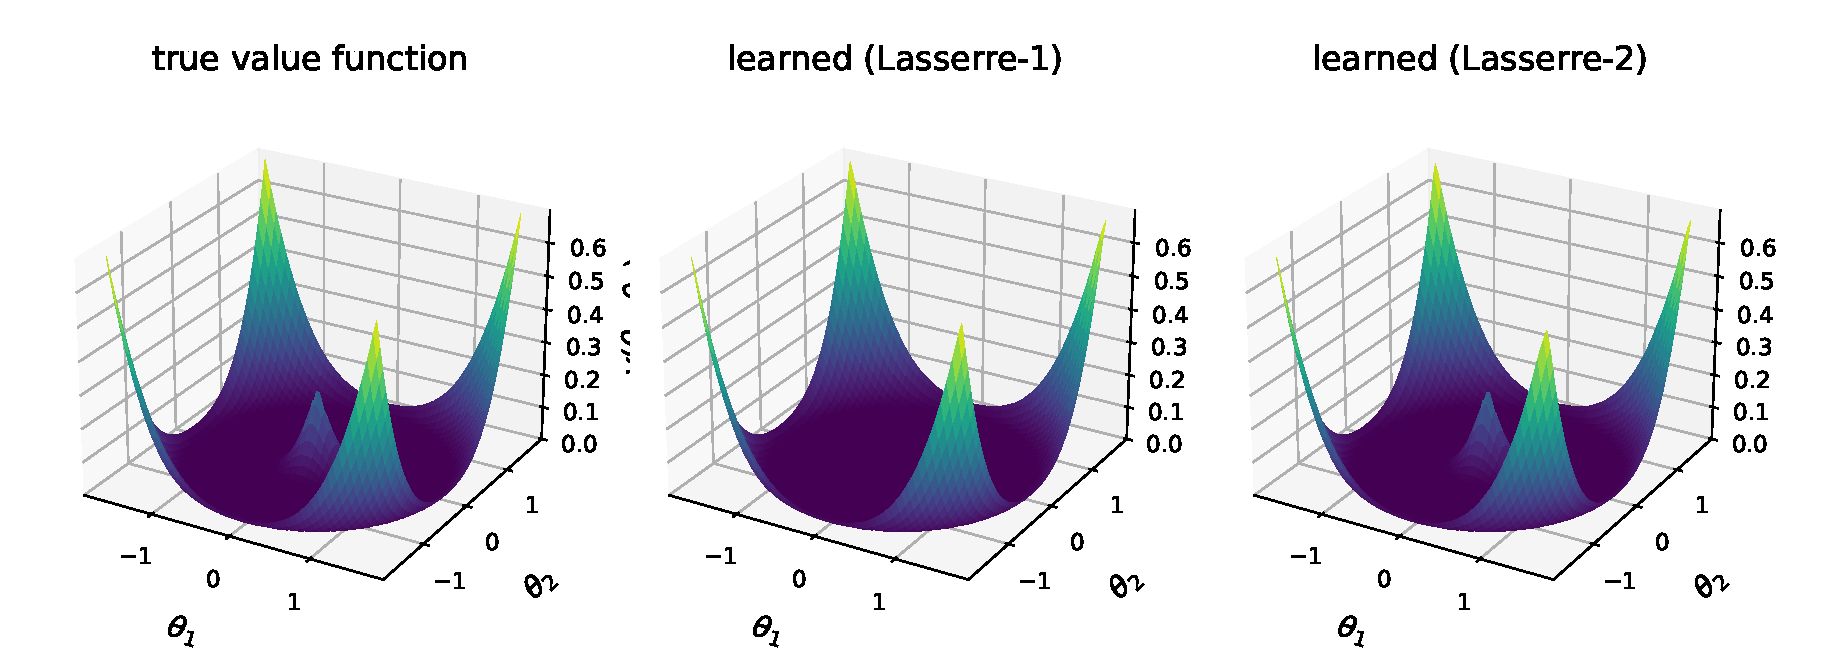
\includegraphics[width=\linewidth]{figures/ik_value_function_comparison.pdf}
    \caption{The true value function $v(\bm{\theta})$ for the inverse kinematics problem (left) and the neural network's learned approximation $\hat{v}(\bm{\theta})$ trained on the first-order Lasserre (Shor) relaxation (center) and the tighter second-order Lasserre relaxation (right), over target positions $\bm{\theta} = (\theta_1, \theta_2)$. All three panels share a common vertical scale and viewing angle. The flat zero-cost basin is the reachable workspace $|\ell_1 - \ell_2| \le \|\bm{\theta}\| \le \ell_1 + \ell_2$, where the target is attainable exactly, and the central spike is the unreachable region near the origin. Both learned surfaces closely reproduce the true value function, including the sharp central feature.}
    \label{fig:ik-value-function}
\end{figure}

\subsection{Digital Communications: MIMO Detection}

The multiple-input multiple-output (MIMO) detection problem arises in digital communications, where a discrete signal must be recovered from a noisy linear measurement in real-time. A transmitted signal $\mathbf{x} \in \{-1, +1\}^n$ is sent over a fixed, complex-valued channel $H \in \mathbb{C}^{m \times n}$ and corrupted by Gaussian noise into the received signal $\bm{\theta} = H \mathbf{x} + \bm{\epsilon} \in \mathbb{C}^{m}$, which parameterizes the problem. Maximum-likelihood detection recovers $\mathbf{x}$ by minimizing the squared measurement error, yielding the non-convex QCQP
\begin{equation}
\begin{aligned}
    v(\bm{\theta}) ~=~ \min_{x \in \mathbb{R}^n} \quad & \|H \mathbf{x} - \bm{\theta}\|^2 \\
    \text{s.t.} \quad & x_i^2 = 1, \quad i = 1, \ldots, n,
\end{aligned}
\label{prob:MIMO}
\end{equation}
whose $2^n$ feasible points (the candidate transmitted signals) are all local minima.

We convexify problem \cref{prob:MIMO}{}{} via semidefinite relaxation (i.e., the Shor or Lasserre-1 relaxation). We introduce the lifted matrix variable $Y$ such that $Y$ is symmetric positive semidefinite and $Y_{ij}$ replaces $x_i x_j$. We therefore require that $Y_{ii} = 1$ for all $i \in \{1, \dots n\}$ in the constraints.

We fix a random channel matrix with $m = 4$, $n = 2$, sample transmitted signals $x \in \{-1, +1\}^n$ uniformly with noise variance $\sigma^2 = 0.1$, and obtain feasible solutions with a fast zero-forcing detector (a linear pseudo-inverse of $H$ followed by rounding). MIMO detection is among the hardest of our value functions to learn: because the parameter is the noisy received signal, $v(\bm{\theta})$ jumps as $\bm{\theta}$ crosses the maximum-likelihood decision boundaries between candidate signals, so the target is rough rather than smooth. The network's prediction error is consequently large relative to the small spread of the optimal value, which makes the certificate conservative for this problem and results in a high false negative rate. We return to this in Section~\ref{sec:discussion}.

\subsection{Power Systems Optimization: AC Optimal Power Flow}
\label{subsec:acopf-experiment}

The alternating current optimal power flow (AC-OPF) problem is solved by grid operators approximtely every five minutes to schedule generation at minimum cost subject to the physics of the electrical network.
It is a non-convex QCQP parameterized by the real and reactive load $\bm{\theta} = (\mathbf{p}_D, \mathbf{q}_D)$ at each bus.

Let us now write the AC-OPF formulation. Consider a power network with a set of buses $\mathcal{N} = \{0, 1, 2, ..., n\}$, set of generator buses $\mathcal{G} \subseteq \mathcal{N}$, and set of lines $\mathcal{L} \subseteq \mathcal{N} \times \mathcal{N}$. We define the variables, parameters, and expressions associated with bus $k \in \mathcal{N}$ as follows:
\begin{itemize}[itemsep=2pt, topsep=0pt, parsep=0pt, partopsep=0pt]
    \item $v_k = v_{dk} + j\, v_{qk}$: Apparent (real and reactive) voltage.
    \item $p_{Dk} + j\, q_{Dk}$: Real and reactive power demand or load.
    \item $p_{Gk} + j\, q_{Gk}$: Real and reactive power generation.
    \item $f_{Ck}(p_{Gk}) = c_{k2}\, p_{Gk}^2 + c_{k1} \, p_{Gk} + c_{k0}$: Convex quadratic cost function of real power generation.
    \item $f_{vk}(\mathbf{v}_d, \mathbf{v}_q) = v_{dk}^2 + v_{qk}^2$: Squared voltage magnitude.
\end{itemize}

Let $Y = G + j B$ be the bus admittance matrix of an equivalent $\Pi$ circuit model of the network.
The real and reactive power generation at each bus are related to the bus voltages through the power flow equations $p_{Gk} = f_{Pk}(\mathbf{v}_d, \mathbf{v}_q)$ and $q_{Gk} = f_{Qk}(\mathbf{v}_d, \mathbf{v}_q)$, where
{
\setlength{\abovedisplayskip}{1pt}
\setlength{\belowdisplayskip}{3pt}
\setlength{\jot}{0pt}
\setlength{\arraycolsep}{3pt}
\begin{align}
    f_{Pk} :=  p_{Dk} + &v_{dk} \sum_{i=1}^{n}(G_{ki} v_{di} - B_{ki} v_{qi})
    + v_{qk} \sum_{i=1}^n (B_{ki} v_{di} + G_{ki} v_{qi}) \label{eq:active-power-flow}\\
    f_{Qk} := q_{Dk} + &v_{dk}\sum_{i=1}^{n}(-B_{ki} v_{di} - G_{ki} v_{qi})
    + v_{qk} \sum_{i=1}^n (G_{ki} v_{di} - B_{ki} v_{qi}) \label{eq:reactive-power-flow}
\end{align}
}

We may write AC-OPF parameterized by real and reactive power demand $\bm{\theta} = (\mathbf{p}_D, \mathbf{q}_D)$ as follows:
\begin{align}
    v(\bm{\theta}) ~= ~ \min~& \sum_{k \in \mathcal{G}} f_{Ck}(f_{Pk}(\mathbf{v}_d, \mathbf{v}_q))  \label{eq:AC-OPF} \\
    \text{s.t.}~& p_{Gk}^{min} \leq f_{Pk}(\mathbf{v}_d, \mathbf{v}_q) \leq p_{Gk}^{max} \label{constr:max-real-power} \\
    & q_{Gk}^{min} \leq f_{Qk}(\mathbf{v}_d, \mathbf{v}_q) \leq q_{Gk}^{max} \label{constr:max-reactive-power}\\
    & (v_{k}^{min})^2 \leq f_{Vk}(\mathbf{v}_d, \mathbf{v}_q) \leq (v_{k}^{max})^2 \label{constr:voltage-mag} \\
    & v_{q0} = 0 \label{constr:slack-bus}
\end{align}
where constraints are defined for all buses $k \in \mathcal{N}$. Constraints \cref{constr:max-real-power}{}{} and \cref{constr:max-reactive-power}{}{} bound the real and reactive power output at each bus; constraint \cref{constr:voltage-mag}{}{} bounds the voltage magnitude at each bus; and constraint \cref{constr:slack-bus}{}{} fixes the voltage angle of the slack bus to $0$. In the full AC-OPF formulation used in our experiments, the magnitude of apparent power flow on lines is also constrained. We omit these constraints here for brevity.

For each test system we sample real and reactive load $\bm{\theta} = (\mathbf{p}_D, \mathbf{q}_D)$ and solve two convex relaxations of AC-OPF: the second-order cone (SOCP; \citealp{jabr2006radial}) relaxation, and the tighter chordal semidefinite (SDP; \citealp{lavaei2012zero}) relaxation.
Each load profile is generated by a two-level uniform perturbation of the network's nominal demand: a single system-wide scaling factor $\alpha \sim \mathrm{Uniform}(0.6, 1.2)$ is drawn per sample, together with independent per-bus multipliers $\eta_i \sim \mathrm{Uniform}(0.7, 1.3)$, so that $p_{Di} = \alpha\,\eta_i\,p_{Di}^{0}$ and $q_{Di} = \alpha\,\eta_i\,q_{Di}^{0}$, with the same $\eta_i$ applied to real and reactive demand at bus $i$. 
The system-wide scaling factor captures a wide range of operating conditions, while the per-bus noise diversifies the demand pattern.
Feasible solutions are obtained with an interior point method solver (IPOPT).
The two convex relaxations again trade off computational cost for tightness: the SOCP is loose but fast to solve, whereas the chordal SDP tighter but far slower (Table~\ref{tab:combined}).
Because the true optimal value of AC-OPF is often intractable, we treat the chordal SDP relaxed optimal value as ground truth (for \texttt{case2869pegase}, whose SDP relaxation is also intractable at our time budget, we use the SOCP relaxed optimal value as ground truth). We study eight standard IEEE and PEGASE systems ranging from $9$ buses to $2{,}869$ buses (see Table \ref{tab:acopf-cases}).

\begin{table}[t]
\centering
\caption{AC-OPF test systems used in our experiments.}
\label{tab:acopf-cases}
\begin{tabular}{l rrr rrr}
\toprule
System & Buses & Lines & Gens & \multicolumn{3}{c}{Demand (MW)} \\
\cmidrule(lr){5-7}
 & & & & nominal & min & max \\
\midrule
\texttt{case9} & 9 & 9 & 3 & 315 & 132 & 491 \\
\texttt{case14} & 14 & 20 & 5 & 259 & 109 & 404 \\
\texttt{case39} & 39 & 46 & 10 & 6254 & 2627 & 9757 \\
\texttt{case89pegase} & 89 & 206 & 12 & 8159 & 3427 & 12727 \\
\texttt{case118} & 118 & 179 & 54 & 4242 & 1782 & 6618 \\
\texttt{case300} & 300 & 409 & 69 & 23848 & 10016 & 37202 \\
\texttt{case1354pegase} & 1354 & 1710 & 260 & 74146 & 31141 & 115668 \\
\texttt{case2869pegase} & 2869 & 3968 & 510 & 138935 & 58353 & 216739 \\
\bottomrule
\end{tabular}
\end{table}

\subsection{Integer Programming: Robust 0-1 Knapsack}

The classical 0-1 knapsack problem selects items of value $\mathbf{c} \in \mathbb{R}^n$ and weight $\mathbf{w} \in \mathbb{R}^n$ to maximize their total value subject to a budget constraint $\mathbf{w}^\top \mathbf{x} \leq b$, where $\mathbf{x} \in \{0, 1\}^n$.
The \textit{robust} 0-1 knapsack problem is a variant that considers \textit{uncertain} weights $\mathbf{w} \in \mathcal{U}(\bm{\theta})$ belonging to a parametric uncertainty set.
Here, we specifically consider \textit{ellipsoidal} uncertainty sets with a fixed shape matrix $\bm{\Sigma} \succ 0$ and a varying center $\bm{\theta} = \bm{\mu} \in \mathbb{R}^{n}$,
\begin{align*}
    \mathcal{U}(\bm{\theta}) ~=~ \{ \bm{\mu} + \bm{\Sigma}^{1/2} \, \bm{\zeta} : \| \bm{\zeta} \| \leq \rho \},
\end{align*}
where $\rho > 0$ is a fixed uncertainty budget. In robust 0-1 knapsack, the weight budget constraint must hold for every weight vector in the ellipsoidal uncertainty set:
\begin{equation}
\begin{aligned}
    v(\bm{\theta}) ~=~ \max_{x} \quad & \mathbf{c}^\top \mathbf{x} \\
    \text{s.t.} \quad & \mathbf{w}^\top \mathbf{x} \leq b \quad \forall ~ \mathbf{w} \in \mathcal{U}(\bm{\theta}) \\
    & \mathbf{x} \in \{0, 1\}^n
\end{aligned}
\label{prob:knapsack}
\end{equation}
Unlike other experiments, we do not seek a convex relaxation for problem \cref{prob:knapsack}{}{}. That is because this problem admits an exact reformulation as a mixed-integer second-order cone program (MI-SOCP):
\begin{equation}
\begin{aligned}
    v(\bm{\theta}) ~=~ \max_{x} \quad & \mathbf{c}^\top \mathbf{x} \\
    \text{s.t.} \quad & \bm{\mu}^\top \mathbf{x} + \rho\,\|\bm{\Sigma}^{1/2}\mathbf{x}\| \leq b, \quad \mathbf{x} \in \{0,1\}^n
\end{aligned}
\label{prob:knapsack-socp}
\end{equation}
This type of convex mixed integer nonlinear program that can be solved via standard techniques such as branch-and-bound. However, in real-time settings (such as in high-frequency trading), it may be necessary to use fast heuristics such as the greedy algorithm to obtain approximate solutions to problem \cref{prob:knapsack-socp}{}{}.

In our experiment, we consider robust 0-1 knapsack with $n=25$ items. The item values $\mathbf{c}$ (fixed, drawn once from $\mathrm{Uniform}(20, 30)$), the budget $b = \tfrac{1}{2}\sum_i c_i$, the robustness parameter $\rho = 1$, and the shape matrix
\begin{align*}
    \bm{\Sigma} ~=~ \tau^2 \big[ (1 - \gamma) \mathbf{I} + \gamma \, \mathbf{1}\mathbf{1}^\top \big], \qquad \tau = 5, ~~ \gamma = 0.8,
\end{align*}
are held constant across all instances, so that the only quantity varying across instances is the ellipsoid center: $\bm{\theta} = \bm{\mu} \in \mathbb{R}^{25}$. Each instance draws $\bm{\mu} \sim \mathcal{N}(\mathbf{c}, \bm{\Sigma})$, centering the nominal weights on the values so that more valuable items are also heavier on average and the selection problem is genuinely combinatorial.

The correlation $\gamma$ deserves comment, because it is what makes this experiment informative. If the entries of $\bm{\theta}$ are drawn independently, the optimal value concentrates sharply: $v(\bm{\theta})$ is a sum over the $\sim\!n/2$ selected items, whose independent fluctuations average out, leaving a coefficient of variation of only a few percent and a value function that is essentially a constant plus combinatorial noise. A positive pairwise correlation defeats this averaging by introducing a common factor---all weights are heavy together, tightening the budget, or light together, loosening it---so the total weight that fits, and hence $v(\bm{\theta})$, varies substantially across instances. At $\gamma = 0.8$ the coefficient of variation of $v$ is $0.167$, roughly four times its value in the independent case, while the greedy heuristic still finds the global optimum on only $7.4\%$ of instances, leaving a large and genuinely suboptimal negative class to discriminate.

For each instance we solve problem \cref{prob:knapsack-socp}{}{} to certified global optimality with a branch-and-bound solver from Gurobi \citep{gurobi}, and we additionally solve its continuous relaxation ($\mathbf{x} \in [0,1]^n$), a second-order cone program, with CLARABEL \citep{clarabel}. This yields two candidate learning targets: the exact optimal value $v(\bm{\theta})$, which is discontinuous in $\bm{\theta}$, and the relaxation value $v_r(\bm{\theta}) \geq v(\bm{\theta})$, which is continuous and therefore easier to fit, at the price of a relaxation gap that adds directly to the certificate's slack. We report both.
The fast solver we certify is a greedy heuristic that ranks items by their value-to-nominal-weight ratio $c_i / \mu_i$ in descending order and adds them one at a time, keeping each addition only so long as the robust capacity constraint $\bm{\mu}^\top \mathbf{x} + \rho\,\|\bm{\Sigma}^{1/2}\mathbf{x}\| \le b$ remains satisfied.
Because the value function of a combinatorial problem is comparatively hard to learn, we repeat the experiment with $20{,}000$ and $80{,}000$ training instances, the smaller set being a subset of the larger.

% NOTE: branch-and-bound acceleration experiment (using v_hat to prune/early-stop)
% is a separate workstream, still under analysis; not included in the tables above.

% We now present results from several experiments in which we applied our approach to non-convex optimization problems from power systems, digital communications, and integer programming.
% The purpose of these experiments is to demonstrate the viability of our framework in diverse problem settings.
% Additional information and details may be found in Appendix \ref{sec:experiments-details}.

% \subsection{Input-Convex and Scale-Invariant Neural Networks}

% In each experiment, we trained neural networks to approximate the value functions of parametric optimization problems. In some cases, the value functions possess geometric properties like convexity and scale invariance (positive homogeneity) that may also be enforced in the neural networks, for example, by constraining the weights and biases of the network to take certain values (see Appendix \ref{app:nn-architecture}). 

% % While our framework does not require convex or scale invariant value functions, these properties may be exploited to provide better performance guarantees. In particular, input-convex neural networks (ICNNs) \citep{pmlr-v70-amos17b} have relatively strong performance guarantees compared to generic deep neural networks (DNNs) for approximating convex functions \cite{rosemberg2024learning}. Throughout our experiments, we explored ICNNs' ability to approximate convex value functions. We also prove novel error bounds and performance guarantees for ICNNs in Appendix \ref{app:icnn-guarantees}.

% \subsection{Power Systems Optimization}

% The alternating current optimal power flow (AC-OPF) problem is solved by power system operators approximately every 5 minutes to minimize cost while balancing demand and generation. It is one of the most fundamental optimization problems in power systems. AC-OPF explicitly represents the steady-state physics of AC electricity networks, which are expressed as nonlinear equations relating nodal voltages and power injections (see formulation in Appendix \ref{sec:experiments-details}). These yield quadratic equality constraints in the formulation, which makes AC-OPF a special case of non-convex QCQP.

% \citet{lavaei2012zero} derive a sufficient condition for exactness of the SDP relaxation of AC-OPF, which holds for many real-world power systems. However, solving the SDP relaxation of AC-OPF is often much slower than using machine learning-based solvers or local search methods, especially in large power systems. SDP relaxation is thus seldom used in real-time power system operations. However, by learning to approximate the value function of the SDP relaxation of AC-OPF, one may obtain optimality certificates for faster solvers which lack optimality guarantees on their own. This is the motivation for our experiment.

% \begin{table*}[t]
% \centering
% \caption{Results of AC-OPF experiments. Value function approximation error for DNNs and ICNNs for different IEEE cases and experiment configurations. Results with $<0.01\%$ error are marked with a long dash ``---."}
% %\begin{adjustbox}{width=\textwidth}
% \begin{tabular}{*{3}{c} *{6}{c}}
% \toprule
% \textbf{IEEE Case} & \textbf{Data Dim.} & \textbf{\# Samples} &
% \multicolumn{2}{c}{\textbf{Avg. Pct. Error}} &
% \multicolumn{2}{c}{\textbf{Max. Pct. Error}} \\
% \cmidrule(lr){4-5} \cmidrule(lr){6-7}
% & & & \textbf{DNN} & \textbf{ICNN} & \textbf{DNN} & \textbf{ICNN} \\
% \midrule
% \texttt{ieee9}   & 1  & 5000  & ---      & ---            & $0.02\%$ & $0.01\%$       \\
%          & 3  & 5000  & ---      & ---            & $0.55\%$ & $1.25\%$       \\
%          & 6  & 10000 & $0.04\%$ & ---            & $2.22\%$ & $4.19\%$       \\
% \addlinespace \hline \addlinespace
% \texttt{ieee14} & 3  & 5000  & ---      & ---            & $0.54\%$ & $1.62\%$       \\
%          & 6  & 10000 & ---      & ---            & $0.53\%$ & $2.43\%$       \\
%          & 10 & 20000 & ---      & ---            & $0.21\%$ & $0.41\%$       \\
% \addlinespace \hline \addlinespace
% \texttt{ieee30}  & 6  & 10000 & ---      & ---            & $0.39\%$ & $1.04\%$       \\
%          & 10 & 20000 & ---      & ---            & $0.26\%$ & $0.90\%$       \\
%          & 25 & 50000 & ---      & ---            & $0.13\%$ & $0.58\%$       \\
% \addlinespace \hline \addlinespace
% \texttt{ieee118} & 10 & 20000 & $0.03\%$ & ---            & $0.96\%$ & $0.29\%$       \\
%          & 25 & 50000 & ---      & ---            & $0.13\%$ & $0.53\%$       \\
% \addlinespace \hline \addlinespace
% \texttt{ieee300} & 60 & 30000 & ---      & ---            & $0.55\%$ & $0.53\%$    \\
% \bottomrule
% \end{tabular}
% %\end{adjustbox}
% \label{tab:ACOPF-results}

% \end{table*}

% For several IEEE test power systems, we trained DNNs and ICNNs to approximate the value function of AC-OPF parameterized by real and reactive load at each bus. We obtained training and testing data by solving exact SDP relaxations of AC-OPF. The DNN and ICNN models achieved very low approximation error in our experiments. Maximum error was less than 2-3\% in most experiments, and average error was near-zero. 
% %For reference, the prediction targets (optimal objective function values) in our test data sets had coefficients of variation between 8\% and 45\%, meaning the neural networks achieved good performance relative to the size of the variance of the data. 
% Furthermore, the approximation error was relatively consistent across test cases of widely varying size and data dimension, which indicates that our approach can scale well to larger power systems.
% %In our experiments, IPOPT never converged to a spurious local minimum, though in many instances (30\%) of the \texttt{ieee300} case it outright failed to converge to a feasible solution.
% %This highlights the sensitivity of local search methods to the choice of initial point in non-convex problems.
% Furthermore, our timing comparison results (Table \ref{tab:method-time}) show unsurprisingly that neural network inference is orders of magnitude faster than solving AC-OPF via convexification or local search. Overall, the results suggest that neural networks can quickly and reliably certify optimality of AC-OPF solutions.

% \subsection{Digital Communications}

% The MIMO detection problem, which is an instance of QCQP with complex variables, arises in many signal processing applications. Typically, MIMO detection must be solved for rapidly time-varying signal and channel parameters. Although convexification methods like SDP relaxation have been used to solve MIMO detection, they are typically too slow to be used in practice. Several heuristics have been developed to approximately (sub-optimally) solve MIMO detection in realistic online settings. In \citet{samuel2017deep}, the authors developed a machine learning-based solver for the MIMO detection problem, which achieved good performance. However, heuristic and machine learning-based approaches lack optimality guarantees and may benefit from neural network optimality certificates.

% %The value function $\tilde{v}(y)$ is neither convex nor scale invariant, and therefore we did not attempt to train an ICNN or SINN to learn the value function in our experiments. 
% We solved 5000 instances of the SDP relaxation of MIMO detection with randomly generated noisy signals $\bar{y}$. We certified the exactness of each SDP instance by testing whether a rank-1 solution was obtained. 
% %None of the problem instances failed this test. 
% We trained a DNN to approximate the value function using the Adam optimizer with a learning rate of 0.01 over 3000 epochs. The trained DNN achieved near-zero training loss, and $\mathbf{0.3\%}$ \textbf{average / }$\mathbf{2.5\%}$ \textbf{maximum} error over the test data set of $1500$ points. The trained DNN can therefore reliably certify optimality of detected digital signals.

% \subsection{Integer Programming}


% {
% \setlength{\tabcolsep}{10pt}
% \begin{table}[t]
% \centering
% \caption{Time to solve or predict the optimal cost of 100 AC-OPF instances of \texttt{ieee300}. Experiments were conducted on a 2024 MacBook Air equipped with an 8-core Apple M3 chip and 8 GB of unified memory.}
% \begin{tabular}{lcc}
% \hline
% \textbf{Problem} & \textbf{Software} & \textbf{ Time} \\
% \hline
% AC-OPF SDP & CVXOPT & 30m 55s \\
% AC-OPF & IPOPT &9m 3s  \\
% DNN Inference & PyTorch & 0.1s \\
% \hline
% \end{tabular}
% \label{tab:method-time}

% \end{table}
% }
% \setlength{\tabcolsep}{3pt} 
% \begin{table}[t]
% \centering
% \caption{Results of 0-1 knapsack experiments. Each block shows the results of a different set of experiments.}
% \begin{tabular}{lcc}
% \multicolumn{3}{c}{\textbf{10 Item Knapsack}:  data dim. = 5,~ \# samples = 50000}\\
% \midrule
% \textbf{Network~~} & \textbf{Avg. Pct. Error} & \textbf{Max. Pct. Error} \\
% \midrule
% DNN   & 0.27\% & 2.29\% \\
% ICNN  & 0.02\% & 2.12\% \\
% SINN  & 0.30\% & 3.87\% \\
% CSINN & \textbf{0.01\%} & \textbf{0.56\%} \\
% \addlinespace
% \addlinespace
% \multicolumn{3}{c}{\textbf{30 Item Knapsack}: data dim. = 8,~ \# samples = 80000} \\
% \midrule
% \textbf{Network~~} & \textbf{Avg. Pct. Error} & \textbf{Max. Pct. Error} \\
% \midrule
% DNN   & 1.32\% & 8.88\% \\
% ICNN  & \textbf{0.10\%} & \textbf{0.92\%} \\
% SINN  & 1.20\% & 15.67\% \\
% CSINN & 0.50\% & 5.02\% \\
% \bottomrule
% \end{tabular}
% \vspace{-1em}
% \label{tab:knapsack-results}

% \end{table}

% In this experiment, we trained neural networks to certify optimality of the 0-1 knapsack problem parameterized by the cost vector $c \in \mathbb{R}^n_+$. We solved thousands of problem instances using Gurobi's MI-SOCP linear program solver \citep{gurobi} to obtain data sets for our experiments. We trained a variety of neural network architectures, including DNNs, ICNNs, and scale-invariant and convex scale-invariant networks (SINNs and CSINNs) to approximate the value function. We measured the average and maximum approximation error of each network in each experiment.
% The results are summarized in Table \ref{tab:knapsack-results}.

% The average performance of ICNNs and CSINNs was substantially better than DNNs and SINNs, indicating that special neural network architectures can reduce overfitting and improve performance.
% The good performance of ICNNs and CSINNs in our experiments highlights the potential to integrate neural networks into other solvers. For example, neural networks may be used to certify optimality of linear relaxations of integer programs, or speed branch-and-bound by pruning branches whose objective function value exceeds the network's prediction by a pre-determined threshold.

% % Since $v(c)$ is scale invariant (i.e. positively homogeneous), by Euler's theorem it also satisfies
% {
% \setlength{\abovedisplayskip}{6pt}
% \setlength{\belowdisplayskip}{6pt}
% \setlength{\jot}{0pt}
% \setlength{\arraycolsep}{3pt}
% \begin{align*}
%     v(c) = \nabla v(c)^Tc
% \end{align*}
% }
% Let $x^*(c)$ denote an optimal solution of \eqref{eq:knapsack}, which we assume to be unique. Note that for a particular $i \in \{1, ..., n\}$, we have
% {
% \setlength{\abovedisplayskip}{5pt}
% \setlength{\belowdisplayskip}{8pt}
% \setlength{\jot}{0pt}
% \setlength{\arraycolsep}{3pt}
% \begin{align*}
% \nabla v(c)_i =
% \begin{cases}
% 1 & \text{if } x^*(c)_i = 1, \\
% 0 & \text{if } x^*(c)_i = 0.
% \end{cases}
% \end{align*}
% }
% Therefore, $\nabla v(c) = x^*(c)$ for all $c \in \mathbb{R}^n_+$ such that the corresponding instance of \eqref{eq:knapsack} has a unique solution. Furthermore, if a SINN $\hat{v}(c)$ can approximate the value function to within $\epsilon$ error for all $c \in \Phi \subset \mathbb{R}^n_+$, then
% \begin{align*}
%     |\hat{v}(c) - v(c)| &= \|\nabla \hat{v}(c)^Tc - \nabla v(c)^T c \| \\
%     &\leq \| \nabla \hat{v}(c) - \nabla v(c) \| \cdot \| c\| \leq \epsilon \\
%     \implies& \| \nabla \hat{v}(c) - x^*(c) \| \leq \frac{\epsilon}{\|c\|}
% \end{align*}
% for all $c \in \Phi$ such that $x^*(c)$ is a unique optimal solution of \eqref{eq:knapsack}.
% In other words, by learning to approximate the scale invariant value function of \eqref{eq:knapsack} with a SINN, the gradient of the value function (and therefore an approximate optimal solution mapping) may be indirectly learned as well. The error may also depend on the norm of the cost vector $c$, with larger values of $\|c\|$ generally being preferred. However, due to noise in the training process, the gradient estimator of the trained SINN $\nabla \hat{v}(c)$ is typically not in $\{0, 1\}^n$, and therefore may need to be rounded or projected to obtain feasible a solution to \eqref{eq:knapsack}. Therefore, we propose the following simple approach to compute approximate solutions of the parametric 0-1 knapsack problem using SINNs.
% \begin{algorithm}[H]
% \caption{Approximate 0-1 Knapsack via CSINN}
% \label{alg:approx-knapsack}
% % Unnumbered input/output
% \begin{algorithmic}[0]
% \STATE \textbf{Input:} CSINN $\hat{v}(c)$, cost vector $c \in \mathbb{R}^n$
% \STATE \textbf{Output:} Approximate solution $\hat{x} \in \{0,1\}^n$
% \end{algorithmic}
% % Numbered steps
% \begin{algorithmic}[1]
% \STATE Normalize cost vector: $\hat{c} \gets c / \|c\|$
% \STATE Compute CSINN gradient: $\hat{g} \gets \nabla \hat{v}(\hat{c})$
% \STATE Round to integer solution: $\hat{x} \gets \mathbf{1}(\hat{g} > 0.5)$
% \STATE Ensure feasible solution:
% \end{algorithmic}
% \begin{algorithmic}[0]
% \WHILE{$w^T \hat{x} > b$}
%     \STATE $k \gets \argmin_i \{ \frac{c_i}{w_i} : \hat{x}_i = 1 \} $ \\
%     \STATE $\hat{x}_k \gets 0$
% \ENDWHILE
% \end{algorithmic}
% \end{algorithm}
% This approach may be further improved by using techniques such as Sobolev training \cite{czarnecki2017sobolev}, in which neural networks are trained to approximate both a function's value and its derivatives. It is similar in spirit to the ICNN-based DC-OPF solver developed in \citet{zhang2021convex}, which uses first-order information about the value function to recover optimal solutions from the trained ICNN. However, our algorithm takes advantage of scale invariance of the neural network architecture and does not penalize the gradient error during training. 
% Remarkably, our approximate knapsack solver achieves good performance over the test data set despite never observing optimal knapsack solutions during training. The average (maximum) optimality gap of the CSINN-based solutions was $1.7\%$ ($51.4\%$). The solver returned the globally optimal solution in $78\%$ of test set problem instances.
% Overall, these experiments suggest an interesting new approach to learning optimal solution mappings for 0-1 knapsack and other MILPS.

\subsection{Results}

Table~\ref{tab:combined} reports all results at the fixed operating point $\delta = 3\% \times\mathrm{std.\,}v(\bm{\theta})$ and $\alpha = 0.01$. The offline columns give the mean relaxation value $\bar v_r(\bm\theta)$ the network is trained to predict, the mean true optimal value $\bar v(\bm\theta)$ where tractable, the mean value $\bar f(\hat{\mathbf{x}};\bm\theta)$ achieved by the fast local solver, the network's mean absolute error, and the calibrated conformal offset $\hat q_{99}$ -- the gap between $\bar v_r$ and $\bar v$ is the relaxation gap, and the gap between $\bar f$ and $\bar v$ (or $\bar v_r$, where $\bar v$ is unavailable) is the local solver's mean optimality gap. The online columns give the certification threshold $\delta$ used and the resulting certification counts. Across every experiment the false positive rate is near-zero or close to the $1\%$ target, while the number of certified optima (TP) is high wherever the network is accurate enough that $\hat{q}_{99}$ fits within $\delta$ (AC-OPF, inverse kinematics, QCQP), and low where it is not (MIMO detection, and to a lesser extent robust knapsack), whose rougher value functions the network fits less precisely. The timing columns show the offline solve cost: higher-order relaxations are consistently, and often dramatically, slower, and increasingly so as the system grows---on AC-OPF the chordal SDP costs under $3\times$ the SOCP on \texttt{case9} but is $19$--$107\times$ slower on \texttt{case118}--\texttt{case89pegase}, remaining over $40\times$ slower even on the much larger \texttt{case1354pegase}---whereas a network prediction is sub-microsecond. The local solver, by contrast, does not show a comparably clean scaling trend relative to the SOCP relaxation; we caution against over-reading this comparison given the sample size.

\begin{sidewaystable}[p]
\centering\footnotesize
\caption{All results combined, at the fixed operating point $\delta = 3\%\cdot\mathrm{std}(v(\bm\theta))$
and $\alpha = 1\%$ (offset $q_{99}$), averaged over the four folds. ${}^\ast$AC-OPF is nonconvex and
generally intractable to solve exactly, so genuine $v(\bm\theta)$ is never available there (only
relaxation values of varying tightness); shown as --. SOCP and SDP rows for the same AC-OPF
case are restricted to the subset of instances on which both relaxations converged, so the two
rows describe the identical test population (their $\bar f(\hat{\mathbf{x}};\bm\theta)$ is
therefore always equal, and $\bar v_r$ is guaranteed SDP $\geq$ SOCP, as the relaxation hierarchy
requires); this affects only \texttt{case89pegase}/\texttt{case300}/\texttt{case1354pegase}, where
the two relaxations fail to converge on different instances. Timing: both columns of a given row are
measured identically (like-for-like); the local solver does not depend on the relaxation it is
compared against, so its solve time is measured once per experiment (per AC-OPF case; once for
inverse kinematics) and reused across relaxation rows. For AC-OPF, whose local solver (IPOPT) is
invoked through a file-based modelling interface, we report \emph{solver-internal} time on both
sides (parsed from IPOPT's own timing log for the local column) so the comparison is not dominated
by Python model construction or process-launch overhead. Mean over $50$ random instances per case
(smallest six AC-OPF cases) or $3$--$8$ for \texttt{case1354pegase}/\texttt{case2869pegase}'s SOCP
and \texttt{case1354pegase}'s chordal SDP; non-converged instances excluded from both timing
columns. \textsuperscript{$\dagger$}For \texttt{case2869pegase}'s chordal SDP, only $1$ of $5$
attempted instances converged (each costing $\sim\!70$s regardless of outcome); we report that
single solve time rather than assert a stable average, and omit its offline/online columns
entirely since no certification was computed for it, consistent with treating this relaxation as
effectively intractable at scale (\S\ref{subsec:acopf-experiment}).}
\label{tab:combined}
\resizebox{\linewidth}{!}{%
\begin{tabular}{lll rrr rr r rrrr rr}
\toprule
& & & \multicolumn{5}{c}{Offline} & \multicolumn{5}{c}{Online} & \multicolumn{2}{c}{Timing} \\
\cmidrule(lr){4-8}\cmidrule(lr){9-13}\cmidrule(lr){14-15}
\textbf{Experiment} & \textbf{Relaxation} & \textbf{Case} &
$\bar v_r(\bm\theta)$ & $\bar v(\bm\theta)^\ast$ & $\bar f(\hat{\mathbf{x}};\bm\theta)$ & MAE & $q_{99}$ &
$\delta$ & TP & FP & TN & FN &
Relax.\ Solve & Local Solve \\
\midrule
  \multirow{1}{*}{QCQP} & Shor &  & 2.65 & 2.65 & 12.4 & 0.0022 & 0.012 & 0.14 & 2524 & 0 & 2474 & 2 & 96.1 ms & 94.7 ms \\
\midrule
  \multirow{2}{*}{Inverse Kinematics} & Shor &  & 0.036 & 0.039 & 0.05 & 7.7e-05 & 5.5e-04 & 0.0028 & 4533 & 0 & 193 & 267 & 0.36 ms & 12.4 ms \\
   & Lasserre-2 &  & 0.039 & 0.039 & 0.05 & 8.4e-05 & 5.3e-04 & 0.0028 & 4799 & 0 & 193 & 1 & 34.5 ms & 12.4 ms \\
\midrule
  \multirow{1}{*}{MIMO Detection} & Shor &  & 0.79 & 0.79 & 0.8 & 0.002 & 0.0071 & 0.012 & 96 & 0 & 4 & 4900 & 92.8 ms & 0.14 ms \\
\midrule
  \multirow{16}{*}{AC-OPF} & SOCP & \texttt{case9} & 4,692 & -- & 4,692 & 0.72 & 2.79 & 43.6 & 5000 & 0 & 0 & 0 & 1.80 ms & 4.40 ms \\
   & SOCP & \texttt{case14} & 7,049 & -- & 7,054 & 2.82 & 17.5 & 57.2 & 4999 & 0 & 0 & 1 & 0.60 ms & 3.60 ms \\
   & SOCP & \texttt{case39} & 33,515 & -- & 33,526 & 33.2 & 219 & 376 & 4542 & 0 & 0 & 109 & 2.40 ms & 20.6 ms \\
   & SOCP & \texttt{case89pegase} & 7,275 & -- & 7,281 & 2.52 & 19.4 & 42.4 & 4698 & 0 & 0 & 75 & 10.4 ms & 18.7 ms \\
   & SOCP & \texttt{case118} & 113,180 & -- & 113,454 & 27.8 & 270 & 861 & 4952 & 0 & 0 & 48 & 6.80 ms & 19.8 ms \\
   & SOCP & \texttt{case300} & 582,719 & -- & 583,758 & 252 & 2,325 & 3,925 & 3702 & 0 & 9 & 232 & 20.0 ms & 41.0 ms \\
   & SOCP & \texttt{case1354pegase} & 67,649 & -- & 67,699 & 4.17 & 18.4 & 398 & 3844 & 0 & 0 & 0 & 128 ms & 247 ms \\
   & SOCP & \texttt{case2869pegase} & 126,542 & -- & 126,802 & 7.98 & 33.2 & 731 & 2957 & 0 & 259 & 0 & 349 ms & 467 ms \\
   & SDP & \texttt{case9} & 4,692 & -- & 4,692 & 0.73 & 2.71 & 43.6 & 5000 & 0 & 0 & 0 & 2.10 ms & 4.40 ms \\
   & SDP & \texttt{case14} & 7,054 & -- & 7,054 & 2.94 & 18.2 & 57.2 & 5000 & 0 & 0 & 0 & 5.00 ms & 3.60 ms \\
   & SDP & \texttt{case39} & 33,522 & -- & 33,526 & 30.8 & 196 & 376 & 4584 & 0 & 0 & 67 & 27.4 ms & 20.6 ms \\
   & SDP & \texttt{case89pegase} & 7,281 & -- & 7,281 & 2.52 & 19.1 & 42.4 & 4745 & 0 & 0 & 28 & 1.10 s & 18.7 ms \\
   & SDP & \texttt{case118} & 113,452 & -- & 113,454 & 28.4 & 281 & 861 & 4995 & 0 & 0 & 5 & 128 ms & 19.8 ms \\
   & SDP & \texttt{case300} & 583,523 & -- & 583,758 & 237 & 1,485 & 3,925 & 3894 & 0 & 9 & 39 & 787 ms & 41.0 ms \\
   & SDP & \texttt{case1354pegase} & 67,693 & -- & 67,699 & 4.85 & 19.4 & 398 & 3844 & 0 & 0 & 0 & 8.28 s & 247 ms \\
   & SDP & \texttt{case2869pegase} & -- & -- & -- & -- & -- & -- & -- & -- & -- & -- & 40.3 s\textsuperscript{$\dagger$} & 467 ms \\
\midrule
  \multirow{2}{*}{Robust Knapsack} & Exact & \texttt{n=25} & 281 & 281 & 272 & 1.23 & 3.96 & 1.41 & 50 & 4 & 4238 & 708 & -- & 0.0687 ms \\
   & SOCP & \texttt{n=25} & 283 & 281 & 272 & 1.16 & 3.66 & 1.41 & 7 & 1 & 4241 & 751 & -- & 0.0687 ms \\
\bottomrule
\end{tabular}%
}
\end{sidewaystable}


\section{Discussion} \label{sec:discussion}

Our results indicate that our framework achieves its intended purpose of probabilistically certifying global optima in non-convex optimization problems.
In experiments where the deep neural network learns to approximate the value function with high accuracy, it can certify global optima at or below the target 
false positive rate of $1\%$ within only a few percent of the intrinsic spread of the target optimal value.
For problems with more challenging value functions, the certification accuracy improves with larger training data -- illustrating the
``preservation of difficulty'' of certain NP-hard problems.
As a feedforward pass through the neural network takes only milliseconds, the certificates may be deployed to assist fast solvers
(including local search methods, heuristics, or machine learning-based solvers) in real-time settings.

The probabilistic guarantees of our framework rest on \emph{exchangeability} between the
calibration sample and new test instances. This holds when parameters are drawn
i.i.d.\ from a fixed distribution, as in our experiments.
In realistic, time-varying optimization settings, where observed instances of $\bm{\theta}$ may be 
temporally correlated or subject to distribution shift, the marginal coverage of our framework can degrade, 
and the calibrated conformal offset should be refreshed online or replaced by a weighted conformal variant
(where calibration samples are re-weighted to account for covariate shift)~\citep{tibshirani2019conformal}.

Furthermore, coverage probability in split conformal calibration
is \emph{marginal}: it holds on average over $\Theta$, not conditionally at a
particular $\bm{\theta}$, so the error rate may be uneven across the parameter
space. Conformalized quantile regression~\citep{romano2019conformalized}, which
calibrates a learned quantile model rather than a single conformal offset, is a
natural route to approximate conditional coverage and an interesting direction for
future work.

Finally, we also note that the \emph{power} of our certificates is inherited from the
tightness of the convex relaxation used to generate training data.
Intuitively, a large relaxation gap results in an overly conservative certification
threshold. This is because the candidate solution's
objective value $f(\hat{\mathbf{x}}\, ; \bm{\theta})$ is bounded below by $v(\bm{\theta})$,
but the certification threshold is a calibrated probabilistic lower bound for $v_r(\bm{\theta})$.
Since the relaxation gap may also be uneven across the parameter space (as observed in experiment \ref{subsec:IK}),
hence the conservativeness of the certificates (and the false negative rate) may be uneven as well.
Tightening the relaxation (e.g. by moving up a convexification
hierarchy or adding valid inequalities or cutting planes to the formulation) 
directly improves certification accuracy at a stricter optimality tolerance, at the
offline cost of a larger convex relaxation.

\section{Conclusion} \label{sec:conclusion}
In this work, we proposed an innovative framework for real-time optimality certification in non-convex optimization tasks.
Our framework leverages convexification techniques and machine learning to learn the optimal value function of parametric optimization problems.
By functioning as a meta-certification framework, our method is compatible with various convexification schemes as well as various fast, approximate solvers. 
By training neural networks to approximate the optimal value of a convex relaxation, we shift the computational burden from real-time optimization to offline training. 
Under suitable conditions, the convex relaxation provides a tight lower bound on the original non-convex problem, so candidate solutions that are sufficiently close to the predicted optimal value are assured to be near-globally optimal.
By conformalizing our network predictions, we are able to guarantee coverage probability and bound the misclassification rate (under certain assumptions like exchangeability of the data)
Our proposed framework not only expands the applicability of convexification methods to online optimization, but also offers a new conceptual approach to apply learning-based performance guarantees to fast heuristic solvers.
%This methodology not only improves computational efficiency but also offers a theoretical framework for achieving global optimality in previously intractable non-convex optimization tasks. 
Future work will focus on refining machine learning-based optimality certification using conformal quantile regression, and extending this approach to more diverse classes of non-convex problems.


\subsubsection*{Broader Impact Statement}
In this optional section, TMLR encourages authors to discuss possible repercussions of their work,
notably any potential negative impact that a user of this research should be aware of. 
Authors should consult the TMLR Ethics Guidelines available on the TMLR website
for guidance on how to approach this subject.

\subsubsection*{Author Contributions}
If you'd like to, you may include a section for author contributions as is done
in many journals. This is optional and at the discretion of the authors. Only add
this information once your submission is accepted and deanonymized. 

\subsubsection*{Acknowledgments}
Use unnumbered third level headings for the acknowledgments. All
acknowledgments, including those to funding agencies, go at the end of the paper.
Only add this information once your submission is accepted and deanonymized. 

\bibliographystyle{tmlr}
\bibliography{main}

\appendix

\section{Neural Network Ablation Study} \label{app:ablation}

The architecture ($6$ hidden layers of $256$ units) and training budget ($1000$ epochs) used throughout the paper were selected by ablation on the AC-OPF problem, varying one factor at a time and measuring $4$-fold cross-validated prediction accuracy on the SOCP relaxation. We report the mean absolute percent error (MAPE) of $\hat{v}$ against the relaxation value $v_r$, on three test systems spanning two orders of magnitude in size.

Table~\ref{tab:ablation-depth} varies network depth at fixed width. Prediction error falls steeply as the network deepens---for \texttt{case118}, MAPE drops from $8.7\%$ with a single hidden layer to $3.1\%$ with six---and largely plateaus beyond four to six layers, while training cost grows only modestly. We adopt six hidden layers as a point past which additional depth yields diminishing returns. Table~\ref{tab:ablation-epochs} varies the number of training epochs for the chosen $6\times256$ architecture. Error decreases monotonically with the training budget and flattens by roughly $1000$ epochs (e.g.\ \texttt{case118} improves from $1.38\%$ at $1000$ epochs to only $1.29\%$ at $2000$), so we train for $1000$ epochs throughout. Both trends were consistent across the three test systems, and we found the same architecture transferred well to the other problem families without further tuning.

\begin{table}[h]
\centering\footnotesize
\caption{Network-\emph{depth} ablation on AC-OPF (SOCP relaxation): $4$-fold
cross-validated MAPE (\%) of $\hat{v}$ against $v_r$, at fixed width $256$ and $1000$
epochs. Error falls steeply with depth and plateaus by $4$--$6$ hidden layers, which
motivates our choice of six. Train time is for \texttt{case1354} (seconds, all four folds).}
\label{tab:ablation-depth}
\begin{tabular}{c ccc r}
\toprule
\textbf{Hidden layers} & \texttt{case9} & \texttt{case118} & \texttt{case1354} & \textbf{Train (s)} \\
\midrule
  $1$ & 2.92 & 8.68 & 5.87 & 127 \\
  $2$ & 1.19 & 6.93 & 1.83 & 181 \\
  $3$ & 1.07 & 4.65 & 1.05 & 208 \\
  $4$ & 1.04 & 3.74 & 0.74 & 244 \\
  $5$ & -- & 3.43 & 0.74 & 237 \\
  $6$ & -- & 3.12 & 0.72 & 267 \\
\bottomrule
\end{tabular}
\end{table}

\begin{table}[h]
\centering\footnotesize
\caption{Training-\emph{budget} ablation on AC-OPF (SOCP relaxation, $6\times256$
network): $4$-fold cross-validated MAPE (\%) of $\hat{v}$ against $v_r$ versus the number
of training epochs. Error decreases monotonically and largely plateaus by $1000$ epochs,
our chosen budget. Train time is for \texttt{case1354} (seconds, all four folds).}
\label{tab:ablation-epochs}
\begin{tabular}{c cc r}
\toprule
\textbf{Epochs} & \texttt{case118} & \texttt{case1354} & \textbf{Train (s)} \\
\midrule
  $70$ & 4.61 & 1.11 & 90 \\
  $200$ & 3.26 & 0.77 & 256 \\
  $400$ & 2.33 & 0.53 & 517 \\
  $700$ & 1.58 & 0.50 & 630 \\
  $1000$ & 1.38 & 0.45 & 799 \\
  $1500$ & 1.35 & 0.45 & 1256 \\
  $2000$ & 1.29 & 0.46 & 1638 \\
\bottomrule
\end{tabular}
\end{table}



% \section{Additional Background} \label{sec:additional_background}

% \subsection{Machine Learning-Based AC-OPF Solvers}

% Using machine learning to assist in optimization has garnered strong interest in power systems research. Notably, several works contribute machine learning-based AC-OPF solvers, motivated by the growing need to solve large-scale problem instances with time-varying load and renewables \citep{van2021machine, jiang2024advancements}. While practical experience and some theoretical work has shown that spurious local minima may be rare in AC-OPF, it remains an interesting and potentially important challenge to solve AC-OPF efficiently using machine learning tools \citep{zhou2021conditions}. There are also several well-known examples of AC-OPF problems with spurious local solutions \citep{bukhsh2013local}.

% Many machine learning-based solvers, including those developed by \citet{pan2021deepopf} and \citet{singh2021learning}, directly map load and renewables to optimal AC-OPF solutions. \citet{zhang2022learning} use a Lagrangian duality-based approach to learn solution mappings in a more favorable optimization landscape. \citet{zhang2021convex} train input-convex neural networks (ICNNs) to learn the value function of parametric DC-OPF, and exploit linear programming duality to recover optimal solutions from the network predictions. \citet{deka2019learning} train neural networks to classify active constraint sets of DC-OPF problems, from which optimal solutions may be efficiently computed. \citet{baker2019learning} uses machine learning-predicted AC-OPF solutions as warm starts for local search solvers. \citet{rosemberg2024learning} train ICNNs to learn the value function of AC-OPF, though they did not use convexification techniques to certify the optimality of AC-OPF solutions.

% %Machine learning-based solvers have also been developed for other canonical problems in power systems. \citet{chen2020input} use ICNNs to assist in voltage regulation in distribution networks, and \citet{christianson2024fast} use ICNNs to screen contingency scenarios in security-constrained DC-OPF. \citet{pineda2022learning} propose machine learning methods to solve unit commitment problems, and \citet{pineda2024learning} apply machine learning to optimal transmission switching.

% Though many of these approaches achieve good performance, they still lack optimality guarantees (and even feasibility guarantees in some cases). Solutions obtained from machine learning-based solvers must often be projected into the feasible set in a final step. A key challenge is that solution mappings are high dimensional and discontinuous functions that are difficult to approximate \citep{pan2022deepopf}. Certifying optimality of solutions obtained from machine learning-based solvers therefore remains an important challenge.

% \subsection{Special Neural Network Architectures} \label{app:nn-architecture}
% For certain non-convex problems, the value function is convex and/or positive homogeneous. This is not always the case, even for non-convex problems which admit exact convex relaxations. However, when this is the case, it is conceivably desirable to enforce these properties in a neural network trained to approximate the value function. Therefore we turn our attention to input-convex and scale-invariant neural networks (ICNNs and SINNs), which are special neural network architectures that respectively enforce convexity and positive homogeneity in the network outputs \citep{pmlr-v70-amos17b, bamberger2025approximating}.
% % An ICNN is a type of neural network designed to ensure that the output is a convex function of the input~\cite{pmlr-v70-amos17b}. This property is enforced directly in the neural network architecture by restricting certain neural activation functions to be convex and non-decreasing. 
% \begin{figure}[H]
%     \centering
%     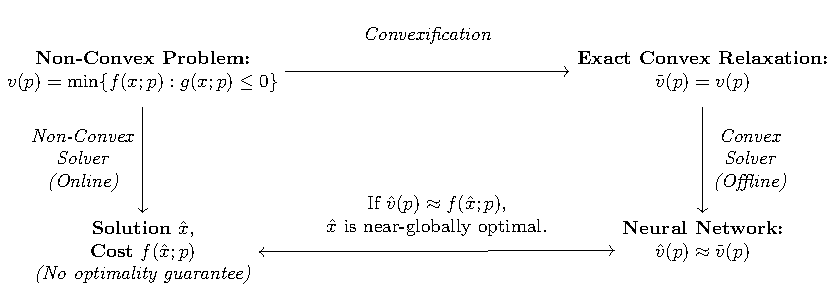
\includegraphics[width=0.7\linewidth]{figures/icnn-figure.pdf}
%     \caption{Neural network with skip connections.}
%     \label{fig:icnn}
% \end{figure}
% Consider a $k$-layer neural network with skip connections and input $y \in \mathbb{R}^d$. For $i=0,\ldots,k-1$ we have
% \setlength{\abovedisplayskip}{7pt}
% \setlength{\belowdisplayskip}{7pt}
% \begin{equation*}
%     z_{i+1} = \sigma_i\left(W^{(z)}_i z_i + W^{(y)}_i y + b_i \right ), \;\; h(y;\theta) = z_k
% \end{equation*}
% % \vspace{-0.5em}
% % \begin{equation}
% % \begin{split}
% % \label{eq-ficnn}
% % %z_1 & = g_0\left(W^{(xy)}_0 \xy + b_0 \right) \\
% % z_{i+1} & = \sigma_i\left(W^{(z)}_i z_i + W^{(y)}_i y + b_i \right ), \;\; h
% % (y;\theta) = z_k
% % \end{split}
% % \vspace{-0.5em}
% % \end{equation}
% where $z_i$ denotes the activation or output of layer $i$, $\theta = \{W^ {(y)}_{0:k-1}, W^{(z)}_{1:k-1}, b_{0:k-1}\}$ are the neural network weights and biases, and $\sigma_i$ are nonlinear activation functions (we define $z_0 = 0$ and $W^{(z)}_0 = 0$ in the input layer). Here, $W^{(z)}_i$ are feedforward connection weights while $W_i^{(y)}$ are skip connection weights and $b_i$ are layer biases. 

% By imposing certain conditions on the activation functions and weights and biases, the function $h(y;\theta)$ can be made to be convex or scale invariant in $y$. In particular:
% \begin{enumerate}
%     \item \textbf{ICNN}: The function $h(y;\theta)$ is convex in $y$ if all feedforward connection weights $W_{1: k-1}^{(z)}$ are non-negative and all activation functions $\sigma_i$ are convex and non-decreasing \citep{pmlr-v70-amos17b}. That is, for all $y_1, y_2 \in \mathbb{R}^d$, $\lambda \in [0, 1]$, we have \[
%     h(\lambda y_1 + (1 - \lambda) y_2; \theta) \leq \lambda h(y_1; \theta) + (1 - \lambda) h(y_2; \theta) \]
%     \item \textbf{SINN}: The function $h(y;\theta)$ is scale invariant (positively homogeneous) if all biases $b_i$ are zero and all activation functions $\sigma_i$ are scale invariant \citep{bamberger2025approximating}. That is, for all $y \in \mathbb{R}^d$, $\lambda \geq 0$, we have \[h(\lambda y; \theta) = \lambda h(y; \theta)\]
% \end{enumerate}

% By enforcing these properties in the neural network architecture, ICNNs and SINNs provide strong inductive bias for learning to approximate convex or positive homogeneous functions. They may achieve lower generalization error and their outputs may be easier to interpret and integrate into optimization frameworks.

% The ReLU activation function ($\text{ReLU}(x) = \max \{0, x\}$) is convex, non-decreasing, and scale invariant, and therefore can be used in both ICNNs and SINNs.

% \section{Experiment Details} \label{sec:experiments-details}

% \subsection{Training Neural Networks}

% Throughout our experiments, we trained deep neural networks to approximate the value functions of non-convex problems. We used a 6-layer architecture whose input dimension $d$ varied by experiment. The five hidden layers had progressively fewer neurons: 512, 512, 256, 64, and 16 neurons. The output layer had a single neuron. For ICNN architectures, skip connections were included between the input layer and hidden layers, while DNNs and SINNs did not have skip connections. However, the number of layers and neurons in each network was the same regardless of architecture.

% To train the neural networks we used a two-stage approach: first, we trained the DNN with stochastic gradient descent (SGD) for 1000-5000 epochs, followed by 1000-5000 epochs of training with Adam. We adopted this two-stage approach because it seemed to be more stable than using either SGD or Adam by itself. 
% The batch size during training ranged from 30-200 samples, and the total size of the data varied between 5000 and 100000 samples in our experiments. 
% In all experiments, the data were split into training (70\%) and test (30\%) data sets.
% Our goal was to achieve zero training loss.

% When training ICNNs and SINNs, the training process was modified. For SINNs, we clamped all biases $b_i$ to zero. For ICNNs, the feedforward connection weights $W^{(z)}_i$ were clipped to be nonnegative after every training iteration. Implementing the clipping step required careful tuning of learning rates to avoid slow convergence (generally, larger learning rates were used to train ICNNs).


% \subsection{Power Systems Optimization}


% We trained neural networks to approximate the value function of AC-OPF parameterized by real and reactive load for several IEEE test power systems (see Table \ref{tab:ieee-description}). Our experimental procedure, which we repeated for each test system, was as follows.

% For a given IEEE test power system with $n$ buses, let $P^{MAX}_D, Q^{MAX}_D \in \mathbb{R}^n$ be vectors of the nominal real and reactive load at each bus. We randomly sampled real and reactive load vectors $\mathbf{p}_D, \mathbf{q}_D$ from $\Phi \subseteq [0, P^{MAX}_D] \times [0, Q^{MAX}_D] \subset \mathbb{R}^{2n}$ and solved the corresponding SDP relaxation of AC-OPF for each instance to obtain the relaxed optimal cost $\tilde{v}(\mathbf{p}_D, \mathbf{q}_D)$. In particular, we solved the SDP relaxation in \citet{lavaei2012zero} using the solver in \citet{madani2014sdp}. Exactness of each SDP relaxation was ascertained \textit{a posteriori} from the rank of the obtained optimal solution. Any problem instance for which a rank-1 solution was not obtained was discarded from the data set. (These instances made up fewer than $5\%$ of samples in all of our experiments.) The valid samples were split into training (70\%) and test (30\%) data sets. A deep neural network (DNN) and input-convex neural network (ICNN) were separately trained to approximate the value function $v(\mathbf{p}_D, \mathbf{q}_D)$. We measured the average and maximum percentage error of the DNN and ICNN predictions over the test data set. 
% %For comparison, we also solved each test data set problem instance with the interior point solver IPOPT \citep{wachter2006implementation}.
% Experiment configurations and results are reported in Table \ref{tab:ACOPF-results}.

% An important detail of our experiments is that real and reactive load were not sampled from the full-dimensional parameter space. In real power systems, electricity demand at different buses is correlated, and the load data may lie in or near a low-dimensional subspace of the ambient space. For instance, in a system with $n$ load buses, the ambient space has $2n$ dimensions, but the data may lie in an $m$-dimensional subspace of $\mathbb{R}^{2n}$ with $m \ll 2n$. We therefore chose to vary the intrinsic dimension of the load data in our experiments (the intrinsic data dimension in each experiment is given in the ``data dim." column in Table \ref{tab:ACOPF-results}). We hypothesized that neural networks would achieve better performance on data with lower intrinsic dimension . For each test system, we tested multiple configurations of the intrinsic data dimension and number of samples. In each experiment, real and reactive load data was uniformly sampled from a randomly chosen $m$-dimensional subspace $\Phi \subseteq [0, P^{MAX}_D] \times [0, Q^{MAX}_D] \subset \mathbb{R}^{2n}$.

% Let us now write the AC-OPF formulation. Consider a power network with a set of buses $\mathcal{N} = \{1, 2, ..., n\}$, set of generator buses $\mathcal{G} \subseteq \mathcal{N}$, and set of lines $\mathcal{L} \subseteq \mathcal{N} \times \mathcal{N}$. We define the variables, parameters, and expressions associated with bus $k \in \mathcal{N}$ as follows:
% \begin{itemize}[itemsep=2pt, topsep=0pt, parsep=0pt, partopsep=0pt]
%     \item $v_k = v_{dk} +\mathbf{j} v_{qk}$: Apparent (real and reactive) voltage.
%     \item $p_{Dk} + \mathbf{j} q_{Dk}$: Real and reactive power demand or load.
%     \item $p_{Gk} + \mathbf{j} q_{Gk}$: Real and reactive power generation.
%     \item $f_{Ck}(p_{Gk}) = c_{k2} p_{Gk}^2 + c_{k1} p_{Gk} + c_{k0}$: Convex quadratic cost function of real power generation.
%     \item $f_{Vk}(\mathbf{v}_d, \mathbf{v}_q) = v_{dk}^2 + v_{qk}^2$: Squared voltage magnitude.
% \end{itemize}

% Let $\mathbf{Y} = G + \mathbf{jB}$ be the bus admittance matrix of an equivalent $\Pi$ circuit model of the network.
% The real and reactive power generation at each bus are related to the bus voltages through the power flow equations $p_{Gk} := f_{Pk}(\mathbf{v}_d, \mathbf{v}_q)$ and $q_{Gk} := f_{Qk}(\mathbf{v}_d, \mathbf{v}_q)$, where
% {
% \setlength{\abovedisplayskip}{1pt}
% \setlength{\belowdisplayskip}{3pt}
% \setlength{\jot}{0pt}
% \setlength{\arraycolsep}{3pt}
% \begin{align}
%     f_{Pk} :=  p_{Dk} + &v_{dk} \sum_{i=1}^{n}(G_{ki} v_{di} - B_{ki} v_{qi})
%     + v_{qk} \sum_{i=1}^n (B_{ki} v_{di} + G_{ki} v_{qi}) \label{eq:active-power-flow}\\
%     f_{Qk} := q_{Dk} + &v_{dk}\sum_{i=1}^{n}(-B_{ki} v_{di} - G_{ki} v_{qi})
%     + v_{qk} \sum_{i=1}^n (G_{ki} v_{di} - B_{ki} v_{qi}) \label{eq:reactive-power-flow}
% \end{align}
% }

% We may write AC-OPF parameterized by real and reactive power demand $\mathbf{p}_D$ and $\mathbf{q}_D$ as follows:
% \begin{align}
%     v(\mathbf{p}_D, \mathbf{q}_D) := ~ \min~& \sum_{k \in \mathcal{G}} f_{Ck}(f_{Pk}(\mathbf{v}_d, \mathbf{v}_q))  \label{eq:AC-OPF} \\
%     \text{s.t.}~& \mathbf{p}_{Gk}^{min} \leq f_{Pk}(\mathbf{v}_d, \mathbf{v}_q) \leq \mathbf{p}_{Gk}^{max} \label{constr:max-real-power} \\
%     & \mathbf{q}_{Gk}^{min} \leq f_{Qk}(\mathbf{v}_d, \mathbf{v}_q) \leq \mathbf{q}_{Gk}^{max} \label{constr:max-reactive-power}\\
%     & (V_{k}^{min})^2 \leq f_{Vk}(\mathbf{v}_d, \mathbf{v}_q) \leq (V_{k}^{max})^2 \label{constr:voltage-mag} \\
%     & V_{q0} = 0 \label{constr:slack-bus}
% \end{align}
% where constraints are defined for all buses $k \in \mathcal{N}$. Constraints \eqref{constr:max-real-power} and \eqref{constr:max-reactive-power} bound the real and reactive power output at each bus; constraint \eqref{constr:voltage-mag} bounds the voltage magnitude at each bus; and constraint \eqref{constr:slack-bus} fixes the voltage angle of the slack bus to $0$. In the full AC-OPF formulation used in some of our experiments, the magnitude of apparent power flow on lines may also be constrained. We omit these constraints here for brevity.

% {
% \setlength{\tabcolsep}{15pt}
% \begin{table}[t]
% \centering
% \caption{IEEE test systems used in our AC-OPF experiments \citep{ieeetestcases}.}
% \begin{tabular}{cccc}
% \toprule
% \textbf{IEEE Case} & \textbf{\# Buses}&  \textbf{\# Lines} & \textbf{\# Generators} \\
% \midrule
% \texttt{ieee9}     & 9   & 9  & 3 \\
% \texttt{ieee14}    & 14  & 20  & 5 \\
% \texttt{ieee30}    & 30  & 41  & 6 \\
% \texttt{ieee118}   & 118 & 186  & 54 \\
% \texttt{ieee300}   & 300 & 411  & 69 \\
% \bottomrule
% \end{tabular}
% \label{tab:ieee-description}
% \end{table}
% }

% \subsection{Digital Signal Processing}

% In this experiment, we consider the parametric multi-input multi-output (MIMO) detection problem:
% \begin{align}
%     v(\bar{y}) :=~\min~&\|\bar{y} - \bar{H}x\|_2^2 \label{eq:MIMO-detection}\\
%     \text{s.t.}~& x_i^2 = 1, \quad i=1,...,n \nonumber
% \end{align}
% Here $x \in \{-1, 1\}^n$ is the discrete signal to be detected, $\bar{H} \in \mathbb{C}^{m \times n}$ is a complex-valued channel matrix, and $\bar{y} \in \mathbb{C}^m$ is a complex-valued noisy signal of the form
% \begin{align}
%     \bar{y} = \bar{H} x + \epsilon \label{eq:noisy-signal}
% \end{align}
% where $\epsilon$ is random Gaussian noise. The problem is parameterized by the received signal $\bar{y}$. Observe that any instance of the MIMO detection problem \eqref{eq:MIMO-detection} has $2^n$ feasible points, each of which is a local minimum.

% In our experiment, we randomly generated a fixed channel matrix $\bar{H} \in \mathbb{C}^{m \times n}$ with $m = 4$ and $n = 2$:
% \[
% \bar{H} =\begin{bmatrix}
% ~~~0.70 + \textbf{j}0.41 & ~~~0.40 + \textbf{j}0.11 \\
% -0.41 + \textbf{j}0.62 &-0.80 + \textbf{j}0.12 \\
% ~~~0.67 + \textbf{j}0.01 & -0.02+ \textbf{j}0.52 \\
% -0.42 + \textbf{j}0.28 & -0.28 + \textbf{j}0.76
% \end{bmatrix}
% \]
% We generated $5000$ uniform random instances of the discrete signal $x \in \{-1, 1\}^n$ and noise $\epsilon \sim \mathcal{N}(0, \sigma^2 I_m)$ with $\sigma^2 = 0.1$, from which the received signal was constructed according to \eqref{eq:noisy-signal}. We reformulated \eqref{eq:MIMO-detection} as a QCQP over real variables using the transformation
% \[
% H = \begin{bmatrix} \Re(\bar{H}) \\ \Im(\bar{H}) \end{bmatrix} \in \mathbb{R}^{2m \times n}, \quad
% y = \begin{bmatrix} \Re(\bar{y}) \\ \Im(\bar{y}) \end{bmatrix} \in \mathbb{R}^{2m}.
% \]
% The transformed problem may be written as
% \begin{align}
%     % v(\bar{y}) = \min~& \|\bar{y} - \bar{H}x\|^2_2 = (\bar{y} - \bar{H}x)^T (\bar{y} - \bar{H}x) = \bar{y}^T\tilde{y} - 2 \bar{y}^T \bar{H} x + x^T \bar{H}^T \bar{H} x \\
%     v(y) = \min~& x^T Q x + 2c^T x + r \label{eq:MIMO-transformed} \\
%     \text{s.t.}~& x_i^2 = 1, \quad i = 1, 2, ..., n \nonumber
% \end{align}
% with $Q = H^T H$, $c = -H^T y$ and $r = y^Ty$. The SDP relaxation of \eqref{eq:MIMO-transformed} is
% \begin{align}
%     \tilde{v}(y) := \min~& \langle M, X \rangle \label{eq:MIMO-SDP} \\
%     \text{s.t.}~& X_{ii} = 1, \quad i = 1, 2, ..., n+1 \nonumber \\
%     & X \succeq 0 \nonumber
% \end{align}
% where we have implicitly lifted $x$ to $[x^T ~~~ 1]^T$ and where
% \[
% M = \begin{bmatrix}
%     Q & c \\
%     c^T & r
% \end{bmatrix}
% \]
% We solved the SDP relaxation \eqref{eq:MIMO-SDP} in our experiments to evaluate $\tilde{v}(y)$.

% \subsection{Integer Optimization}

% In this experiment, we consider the parametric 0-1 knapsack problem with $n$ items:
% \begin{align}
%     v(c) :=~\max~& c^Tx \label{eq:knapsack} \\
%     \text{s.t.}~& w^T x \leq b \nonumber \\
%     &x \in \{0, 1\}^n \nonumber
% \end{align}
% Here $c \in \mathbb{R}^n_+$ is the cost vector, $w \in \mathbb{R}^n_+$ is the weight vector, and $b \in \mathbb{R}_+$ is the knapsack capacity or budget. The problem is parameterized by the cost vector $c$.

% We solved tens of thousands of instances of problem \eqref{eq:knapsack} to develop training data sets for our experiments.
% %We did not explicitly use convexification techniques, although many state-of-the-art MILP solvers benefit from convexification ``under the hood" -- for instance, by using lift-and-project methods to speed branch-and-bound. 
% We considered problems with $n = 10$ and $n = 30$ items. 
% %In a spirit similar to our AC-OPF experiments, 
% Cost vectors were sampled from a subspace of the ambient parameter space $\Phi = [0, 10]^n\subset \mathbb{R}^n_+$. 
% %The subspaces had dimension $m=5$ and $m=8$ for the $10$-item and $30$-item knapsack experiments, respectively, and were chosen randomly. 
% We followed a training procedure similar to our other experiments: data were split into training (70\%) and test (30\%) data sets, and we used both SGD and Adam to train the neural networks for 6000 epochs. We trained a DNN, ICNN, as well as SINN and CSINN (scale-invariant and convex scale-invariant neural network) in each experiment. We measured the average and maximum test set error of each neural network.
% For solving instances of the 0-1 knapsack problem, we did not explicitly use convexification techniques. However, many state-of-the-art MILP solvers do in fact benefit from convexification ``under the hood" -- for instance, by using lift-and-project methods to speed branch-and-bound.

% Note that the value function $v(c)$ in \eqref{eq:knapsack} is convex in $c$, as it is a maximum over a finite number of linear functions in $\mathbb{R}^n$.
% Therefore, for any $c_1, c_2 \in \mathbb{R}^n_+$ and $\lambda \in [0, 1]$ we have
% {
% \setlength{\abovedisplayskip}{2pt}
% \setlength{\belowdisplayskip}{3pt}
% \setlength{\jot}{0pt}
% \setlength{\arraycolsep}{3pt}
% \begin{align*}
%     v(\lambda c_1 + (1- \lambda)c_2) \leq \lambda v(c_1) + (1 - \lambda)v(c_2)
% % \end{align*}
% % }
% It is also scale invariant, as scaling the cost vector by a positive constant does not change the optimal solution and only proportionally scales the optimal objective function value.
% %That is, for all $c \in \mathbb{R}^n_+$ and $\lambda > 0$ we have
% % {
% % \setlength{\abovedisplayskip}{2pt}
% % \setlength{\belowdisplayskip}{3pt}
% % \setlength{\jot}{0pt}
% % \setlength{\arraycolsep}{3pt}
% % \begin{align*}
% %     v(\lambda c) =\lambda v(c)
% % \end{align*}
% % }
% We therefore explored training DNNs, ICNNs, SINNs, and CSINNs to learn the value function $v(c)$ in this experiment.

% In this experiment, we also explored the potential to obtain optimal solution mappings from the trained neural networks. Since $v(c)$ is scale-invariant, it satisfies the equation $v(\lambda c) = \lambda v(c)$ for all $\lambda \geq 0$. Therefore,
% \begin{align*}
% v(c) &= \nabla v(c)^T c
% \end{align*}
% for all $c \in \mathbb{R}^n_+$ where $\nabla v(c)$ is well-defined (i.e., when \eqref{eq:knapsack} has a unique solution $x^*(c) \in \{0, 1\}^n$). Therefore, for such a $c \in \mathbb{R}^n_+$, it can be seen that $\nabla v(c) = x^*(c)$. Therefore, if the gradient of a trained neural network $\hat{v}(c)$ approximates the gradient of $v(c)$ well, then $\nabla \hat{v}(c)$ may approximate an optimal solution mapping for \eqref{eq:knapsack}. We conducted experiments in which we used the gradient of the trained CSINN $\hat{v}(c)$ to obtain approximate 0-1 knapsack solutions by rounding / projecting $\nabla \hat{v}(c)$ to the feasible set of \eqref{eq:knapsack}. We were able to recover optimal solutions in over 70\% of test problem instances for the 10-item knapsack problem. This method could likely be further improved via Sobolev training of the CSINN, which is a method of controlling gradient approximation error during training \citep{czarnecki2017sobolev}.

% \section{Approximation Error Bounds and ICNN Performance Guarantees} \label{app:icnn-guarantees}

% There are two ways in which we may bound the approximation error of $\hat{v}(p)$: one-sided and two-sided error bounds.

% \begin{definition}
%     A \textbf{\textit{one-sided error bound}} only bounds the error in one direction. It is a bound of the form
%     \[
%     \hat{v}(p) - v(p) \leq B \quad \forall~ p \in \Phi.
%     \]
%     Given this one-sided error bound, one may always conclude that if $\hat{x}$ is feasible for \eqref{eq:parametric_opt} then 
%     \[
%     f(\hat{x};p) - v(p) \leq f(\hat{x};p) - \hat{v}(p) + B.
%     \]
% \end{definition}

% \begin{definition}
%    A \textbf{\textit{two-sided error bound}} bounds the error in both directions, or the absolute error. It is a bound of the form
%    \[
%    |\hat{v}(p) - v(p)| \leq B \quad \forall~ p \in \Phi.
%    \]
%    Given this two-sided error bound, one may always conclude that if $\hat{x}$ is feasible for \eqref{eq:parametric_opt} then
%    \[
%    f(\hat{x};p) - \hat{v}(p) - B \leq f(\hat{x};p) - v(p) \leq f(\hat{x};p) - \hat{v}(p) + B.
%    \]
% \end{definition}

% In the context of optimality certification, a one-sided error bound allows one to bound the optimality gap from \textit{above}, while a two-sided error bound allows one to bound the optimality gap from \textit{above} and \textit{below}. (The optimality gap is always bounded below by zero as well. However, it is possible to provide a tighter lower bound with a two-sided error bound.)

% As we have stated, the ability of a neural network to certify optimality depends on its ability to approximate the value function well. We introduced the notions of one-sided and two-sided error bounds, which allow one to bound the optimality gap of feasible solutions from one or both directions using the neural network's predictions. 
% %In practice, error bounds are often estimated from validation tests -- i.e., observing the maximum error over a large validation data set that was not used during training, and which is believed to be representative of the true range of $p$ over the parameter space. However, such empirical error bounds do not always suffice when robust performance guarantees are required. We therefore turn our attention to \textit{theoretical} performance guarantees for neural networks.

% Unfortunately, the gap between theory and observation remains quite large when it comes to bounding the error of generic deep neural networks (DNNs). By comparison, input-convex neural networks (ICNNs) \citep{pmlr-v70-amos17b} can have much stronger theoretical performance guarantees for learning to approximate convex functions. We therefore turn our attention to approximating \textit{convex} value functions with ICNNs. We note that the value functions of non-convex problems can be (provably) convex. For instance, if a QCQP parameterized by right-hand side uncertainty always admits an exact SDP relaxation, then its value function is convex (see Appendix \ref{sec:structured-QCQP} for more details).

% \citet{zhang2021convex} studied the approximation abilities of ICNNs in the context of learning to approximate the value function of parametric DC-OPF.
% %Their theorem 6.5 shows that the ICNN gradient within the convex hull of the training data must lie within a bounded polytope if the ICNN achieves zero value error over the training data set (our assumption \ref{ass:zero-val-error} below).
% Furthermore, \citet{rosemberg2024learning} developed a two-sided error bound for ICNNs trained to approximate the value function of a parametric linear program (LP). They show that the the error is bounded over the convex hull of the training data if the ICNN achieves zero value error \textit{and} zero gradient error during training. We derive a similar two-sided error bound but under the weaker assumption of \textit{bounded} gradient error (Assumption \ref{ass:bounded-grad-error} below). We also derive a one-sided error bound when no assumption about the gradient error is made. This is an important generalization, as zero gradient error over the training data is usually not achieved even when zero value error is achieved.

% \subsubsection*{Notation, Assumptions, and Error Bounds}

% Let $v(p)$ denote a convex value function, and $\hat{v}(p)$ denote an ICNN trained to approximate the value function. Note that problem \eqref{eq:parametric_opt} need not be convex for it to have a convex value function. Let $\mathcal{P} = \{p_1, ..., p_N\} \subset \Phi$ denote the training data, with corresponding labels $\{v(p_1), ..., v(p_N)\} \subset \mathbb{R}$. Let $\operatorname{conv}(\cdot)$ denote the convex hull of a set, and let $\operatorname{diam}(\cdot)$ denote the diameter of a set. All norms $\| \cdot \|$ denote the Euclidean norm.

% Furthermore, we define the ``training data simplex" of $p \in \operatorname{conv}(\mathcal{P})$ as follows. The training data simplex $\mathcal{S}(p) \subset \mathcal{P}$ is the minimum diameter subset of the training data that contains $p$ in its convex hull. That is,
% \[
% \mathcal{S}(p) = \arg \min_{\mathcal{S} \subseteq \mathcal{P}} \{ \operatorname{diam(\mathcal{S}) ~:~ p \in \operatorname{conv}(\mathcal{S}} \}.
% \]
% We assume that $\mathcal{S}(p)$ is well defined for all $p \in \operatorname{conv}(\mathcal{P})$ (i.e., there are never ties between subsets of the data). As a corollary of Caratheodory's theorem, $\mathcal{S}(p)$ contains at most $d+1$ training data points.

% %To derive error bounds that come even close to the actual worst-case performance of DNNs and ICNNs, one must introduce assumptions on the function classes under consideration, such as Lipschitz continuity of the value function and/or its derivative(s). These assumptions may not always hold in practice, but they are useful to shed light on generalization abilities. 
% %For instance, the value function of a parametric linear program (LP) is piecewise linear, and therefore is not smooth (its gradient is not Lipschitz continuous), but is itself Lipschitz continuous over a compact domain such as $\Phi$. In our analysis, we use the following assumptions to derive error bounds on $\hat{v}(p)$.

% %A neural network's ability to certify optimality is limited by its ability to approximate the value function.
% %As we have previously stated, if a neural network's approximation error is uniformly bounded by $\epsilon$ over a parameter set $\Phi \subset \mathbb{R}^d$, then it may certify $2\epsilon$-optimality for problem instances in $\Phi$. Therefore, we are interested in provable worst-case performance guarantees for neural networks.

% %Often the maximum prediction error over a validation set is used as an empirical estimate of worst-case performance. However, we are also interested in theoretical performance guarantees, both because they are stronger than empirical estimates and because they may illuminate the robustness of a model's performance. We therefore turn our attention to neural network performance guarantees.

% %For instance, an assumption that is frequently used to derive error bounds is smoothness of the ground truth function. However, the value functions of many parametric optimization problems are not smooth. For example, the value function of a parametric linear program is typically piecewise linear. A more basic assumption that may be satisfied 
% %Nonetheless, the resulting error bounds may be illuminating even if the assumptions are not exactly satisfied in practice.

% %We analyze the following setting. As before, let $v(p)$ be the value function of a parametric optimization problem, and $\hat{v}(p)$ be a neural network trained to approximate $v(p)$. Let $\mathcal{P} = \{p_1, p_2, ..., p_N\} \subset \mathbb{R}^d$ be training data with corresponding labels $\{v(p_1), v(p_2), ..., v(p_N)\}$. Assume that $\mathcal{P} \subset \Phi$, where $\Phi$ is a compact set in $\mathbb{R}^d$. For now, we make the following assumptions.

% % \begin{assumption}[\textit{Lipschitz Continuity}] The value function $v(p)$ is Lipschitz continuous with Lipschitz constant $L$ over its domain $\Phi$. That is, for any $p, q \in \Phi$
% % \[
% % |v(p) - v(q) | \leq L \|p - q\|
% % \]
% % This suffices to bound the gradient of $v(p)$ over $\Phi$:
% % \[
% % \| \nabla v(p) \| \leq L \quad \forall ~ p \in \Phi.
% % \]
% % \end{assumption}

% We now state our main error bound results. Note that these results hold only for points $p \in \operatorname{conv}(\mathcal{P})$, and not arbitrary $p \in \Phi$. This is a common limitation of theoretical performance guarantees for ICNNs, and is difficult to avoid without making stronger assumptions.

% Our first error bound uses the following assumption of zero approximation error over the training data.
% \vspace{0.25em}
% \begin{assumption}[\textit{Zero Value Error}] 
%     The trained neural network approximates the value function with zero error over the training data set. That is,
%     \[
%     \hat{v}(p_i) = v(p_i), \quad i = 1, 2, ..., N.
%     \]
%     \label{ass:zero-val-error}
%     \vspace{-1.5em}
% \end{assumption}
% Under this assumption, we obtain the following one-sided error bound for $\hat{v}(p)$. 
% \vspace{0.25em}
% \begin{theorem}[\textit{One-Sided Error Bound}] 
%     Let $v(p)$ be a convex value function and $\hat{v}(p)$ be an ICNN trained to approximate $v(p)$. If Assumption \ref{ass:zero-val-error} holds, then for any $p \in \operatorname{conv}(\mathcal{P})$ we have
%     \[
%     \hat{v}(p) - v(p) \leq \max_{p_i \in \mathcal{S}(p)} \|\nabla v(p_i)\| \operatorname{Diam(\mathcal{S}(p))}
%     \]
%     where $\mathcal{S}(p)$ is the training data simplex of $p$.
%     \label{thm:one-sided-icnn-performance}
% \end{theorem}
% %\textit{(Proof in Appendix \ref{app:thm-one-sided}.)}

% %\vspace{0.5em}
% We strengthen this result by assuming bounded error of the gradient of $\hat{v}(p)$ over the training data.
% \vspace{0.25em}
% \begin{assumption}[\textit{Bounded Gradient Error}] 
%     The gradient of the trained neural network approximates the gradient of the value function over the training data set with error $\epsilon_i$ such that
%     \[
%     \nabla \hat{v}(p_i) = \nabla v(p_i) + \epsilon_i, \quad i=1,2, ...,N,
%     \]
%     where 
%     \[
%     \|\epsilon_i\| \leq r \| \nabla v(p_i)\|, \quad i = 1, 2, ..., N,
%     \]
%     for some scalar $r \geq 0$.
%     \label{ass:bounded-grad-error}
% \end{assumption}
% Under this additional assumption, we obtain the following two-sided error bound for $\hat{v}(p)$.
% \vspace{0.25em}
% \begin{theorem}[\textit{Two-Sided Error Bound}] 
%     Let $v(p)$ be a convex value function and $\hat{v}(p)$ be an ICNN trained to approximate $v(p)$. If Assumptions \ref{ass:zero-val-error} and \ref{ass:bounded-grad-error} hold, then for any $p \in \operatorname{conv}(\mathcal{P})$ we have
%     \[
%     |\hat{v}(p) - v(p)| \leq (1 + r) \max_{p_i \in \mathcal{S}(p)} \|\nabla v(p_i)\| \operatorname{Diam(\mathcal{S}(p))}
%     \]
%     where $\mathcal{S}(p)$ is the training data simplex of $p$.
%     \label{thm:two-sided-icnn-performance}
% \end{theorem}
% %\textit{(Proof in Appendix \ref{app:thm-two-sided}.)}
% %\vspace{0.5em}

% %Even without any assumption about the gradient error, we obtain a relatively tight one-sided error bound that follows from convexity and the assumption that the ICNN interpolates the training data. 
% %Under the additional assumption that the ICNN approximates the gradient with bounded error over the training data, we obtain a two-sided error bound that grows with the magnitude of the gradient error.
% %Observe that when we assume zero gradient error ($r = 0$ in assumption \ref{ass:bounded-grad-error}), we recover theorem 2 of \citet{rosemberg2024learning}, albeit with a tighter bound as we only maximize over the training data simplex and not the full training data set. 
% %While we feel that zero gradient error is a strong assumption, one may attempt to control the gradient error during training via, e.g., Sobolev training \citep{czarnecki2017sobolev}.
% Theorems \ref{thm:one-sided-icnn-performance} and \ref{thm:two-sided-icnn-performance} are illuminating, as they suggest that one should draw more training samples (and reduce the simplex diameter) in regions where the gradient is large to improve ICNN performance.

% %Generalization theorems are often insightful, as they may suggest that well-trained ICNNs are able to achieve reliably good performance on new problem instances. However, they are of limited use for ensuring good performance of ICNNs in practice, as the error bounds they provide are generally quite loose and depend on strong assumptions that are almost never satisfied. For instance, due to the curse of dimensionality, new problem instances almost never lie in the convex hull of the training data set in high dimensions \citep{balestriero2021learning}. Furthermore, even if an ICNN achieves zero prediction error over the training data ($\hat{v}(p_i) = v(p_i)$ for all $i \in \{1, ..., N\}$), it may not necessarily achieve zero gradient prediction error ($\nabla \hat{v}(p_i) \stackrel{?}{=} \nabla v(p_i)$ for all $i \in \{1, ..., N\}$). It is possible to improve gradient prediction error by penalizing it during training, as in Sobolev training \citep{czarnecki2017sobolev}. However, in practice, neural network performance guarantees should be obtained through rigorous testing of trained models on realistic problem instances. We envision that our approach will primarily be used to obtain such ``approximate" or ``probabilistic" optimality guarantees.

% %We now prove theorems \ref{thm:one-sided-icnn-performance} and \ref{thm:two-sided-icnn-performance} in section \ref{subsec:icnn-guarantees}.

% \subsection{Proof of Theorem \ref{thm:one-sided-icnn-performance}} \label{app:thm-one-sided}

% Suppose $p \in \operatorname{conv}(\mathcal{P})$. Then $\mathcal{S}(p) = \{p_1, ..., p_k\}$ is well-defined and contains $k \leq d+1$ training data points. Since $p \in \operatorname{conv}(\mathcal{S}(p))$ by definition, there exist $\lambda_1, ..., \lambda_k$ such that
% \begin{align}
%     \sum_{i=1}^{k} \lambda_i p_i &= p, \\
%     \sum_{i=1}^{k} \lambda_i &= 1, \text{ and } \\
%     \lambda_1, ..., \lambda_k &\geq 0.
% \end{align}
% From convexity of $\hat{v}(p)$ and Assumption \ref{ass:zero-val-error}, we obtain the upper bound
% \begin{align*}
%     \hat{v}(p) \leq \sum_{i=1}^{k} \lambda_i v(p_i)
% \end{align*}
% from which we obtain the trivial one-sided error bound:
% \begin{align*}
% \hat{v}(p) - v(p) &\leq \sum_{i=1}^{k} \lambda_i v(p_i) - v(p) \\
% & = \sum_{i=1}^{k} \lambda_i (v(p_i) - v(p)).
% \end{align*}
% From convexity of $v(p)$ we also have that
% \begin{align*}
%     v(p_i) - v(p) &\leq \nabla v(p_i)^T(p_i - p) \\
%     &\leq \| \nabla v(p_i) \| \|p_i - p \|.
% \end{align*}
% for all $p_i \in \mathcal{S}(p)$. Substituting back into the previous inequality and maximizing over $p_i \in \mathcal{S}(p)$, we obtain the desired result:
% \begin{align*}
%     \hat{v}(p) - v(p) &\leq \quad \sum_{i=1}^{k} \lambda_i\|\nabla v(p_i)\| \|p_i - p \|  \\
%     &\leq \max_{p_i \in \mathcal{S}(p)} \|\nabla v(p_i)\| \|p_i - p \| \\
%     &\leq \max_{p_i \in \mathcal{S}(p)} \|\nabla v(p_i)\| \operatorname{diam}(\mathcal{S}(p)). \qed
% \end{align*}

% \subsection{Proof of Theorem \ref{thm:two-sided-icnn-performance}} \label{app:thm-two-sided}

% The proof closely follows the proof of theorem \ref{thm:one-sided-icnn-performance}, but we make use of the subgradient inequality for convex functions to obtain a two-sided error bound.

% Suppose $p \in \operatorname{conv}(\mathcal{P})$. Then $\mathcal{S}(p) = \{p_1, ..., p_k\}$ is well-defined and contains $k \leq d+1$ training data points. Since $p \in \operatorname{conv}(\mathcal{S}(p))$ by definition, there exist $\lambda_1, ..., \lambda_k$ such that
% \begin{align}
%     \sum_{i=1}^{k} \lambda_i p_i &= p, \\
%     \sum_{i=1}^{k} \lambda_i &= 1, \text{ and } \\
%     \lambda_1, ..., \lambda_k &\geq 0.
% \end{align}
% From convexity of $v(p)$ and $\hat{v}(p)$ and Assumption \ref{ass:zero-val-error} we obtain the upper bound
% \begin{align*}
%     v(p), \hat{v}(p) \leq \sum_{i=1}^{k} \lambda_i v(p_i).
% \end{align*}
% Furthermore, for any $p_i \in \mathcal{S}(p)$ we also have by convexity that
% \[
% v(p) \geq v(p_i) + \nabla v(p_i)^T(p - p_i)
% \]
% and
% \[
%     \hat{v}(p) \geq \hat{v}(p_i) + \nabla \hat{v}(p_i)^T(p - p_i).
% \]
% Therefore,
% \[
%     v(p), \hat{v}(p) \geq \min\{ v(p_i) + \nabla v(p_i)^T(p - p_i), ~\hat{v}(p_i) + \nabla \hat{v}(p_i)^T(p - p_i)\}.
% \]
% Combining these inequalities, we obtain for each $p_i \in \mathcal{S}(p)$ the two-sided error bound
% \begin{align*}
% |\hat{v}(p) - v(p)| &\leq \sum_{j=1}^{k} \lambda_j v(p_j) -\min\{ v(p_i) + \nabla v(p_i)^T(p - p_i), ~\hat{v}(p_i) + \nabla \hat{v}(p_i)^T(p - p_i)\} \\
% &= \sum_{j=1}^{k} \lambda_j v(p_j) - v(p_i) + \max\{\nabla v(p_i)^T(p_i - p), ~ \nabla \hat{v}(p_i)^T(p_i - p)\}.
% \end{align*}
% Summing these error bounds over $p_i \in \mathcal{S}(p)$ with weights given by $\lambda_1, ..., \lambda_k$, we get
% \begin{align*}
%     |\hat{v}(p) - v(p)| &\leq  \sum_{j=1}^{k} \lambda_j v(p_j) - \sum_{i=1}^{k} \lambda_i v(p_i) + \sum_{i=1}^{k} \lambda_i \max\{\nabla v(p_i)^T(p_i - p), ~ \nabla \hat{v}(p_i)^T(p_i - p)\} \\
%     &= \sum_{i=1}^{k} \lambda_i \max\{\nabla v(p_i)^T(p_i - p), ~ \nabla \hat{v}(p_i)^T(p_i - p)\} \\
%     &\leq \max_{p_i \in \mathcal{S}(p)} \{ \max\{\nabla v(p_i)^T(p_i - p), ~ \nabla \hat{v}(p_i)^T(p_i - p)\} \}, 
% \end{align*}
% where we have maximized over $p_i \in \mathcal{S}(p)$ in the final step. Now we use the identity
% \[
% \max\{a,b\} = \frac{a + b + |a - b|}{2}
% \]
% to obtain 
% \begin{align*}
% \max\{\nabla v(p_i)^T(p_i - p), ~ \nabla \hat{v}(p_i)^T(p_i - p)\} &= \frac{(\nabla v(p_i) + \nabla v(p_i) + \epsilon_i)^T(p_i - p) + |\epsilon_i^T(p_i - p)|}{2} \\
% &\leq \frac{2 \|\nabla v(p_i)\| \|p - p_i\|+ 2 \|\epsilon_i\| \|p - p_i\|}{2} \\
% &= ( \| \nabla v(p_i)\| + \| \epsilon_i\|) \|p - p_i\| \\
% &\leq (1 +r)\|\nabla v(p_i)\| \|p - p_i\|.
% \end{align*}
% We have used Assumption \ref{ass:bounded-grad-error} to decompose the gradient $\nabla \hat{v}(p_i)$ and bound norm of the error $\|\epsilon_i\|$. Substituting back into the previous inequality, we obtain the desired result:
% \[
% |\hat{v}(p) - v(p)| \leq (1+r) \max_{p_i \in \mathcal{S}(p)} \|\nabla v(p_i)\| \operatorname{diam}(\mathcal{S}(p)). \qed
% \]

% %\section{ADDITIONAL EXPERIMENTS}


% %%%%%%%%%%%%%%%%%%%%%%%%%%%%%%%%%%%%%%%%%%%%%%%%%%%%%%%%%%%%%%%%%%%%%%%%%%%%%%%
% %%%%%%%%%%%%%%%%%%%%%%%%%%%%%%%%%%%%%%%%%%%%%%%%%%%%%%%%%%%%%%%%%%%%%%%%%%%%%%%

\end{document}
